%definira klasu dokumenta 
\documentclass[12pt]{report} 

%prostor izmedu naredbi \documentclass i \begin{document} se zove uvod. U njemu se nalaze naredbe koje se odnose na cijeli dokument

%osnovni LaTex ne može riješiti sve probleme, pa se koriste različiti paketi koji olakšavaju izradu željenog dokumenta
\usepackage[croatian]{babel} 
\usepackage{amssymb}
\usepackage{amsmath}
\usepackage{txfonts}
\usepackage{mathdots}
\usepackage{listings}
\usepackage{titlesec}
\usepackage{array}
\usepackage{lastpage}
\usepackage{etoolbox}
\usepackage{tabularray}
\usepackage{color, colortbl}
\usepackage{adjustbox}
\usepackage{geometry}
\usepackage[classicReIm]{kpfonts}
\usepackage{hyperref}
\usepackage{fancyhdr}

\usepackage{graphicx}
\graphicspath{ {./slike/} }

\usepackage{float}
\usepackage{setspace}
\restylefloat{table}


\patchcmd{\chapter}{\thispagestyle{plain}}{\thispagestyle{fancy}}{}{} %redefiniranje stila stranice u paketu fancyhdr

%oblik naslova poglavlja
\titleformat{\chapter}{\normalfont\huge\bfseries}{\thechapter.}{20pt}{\Huge}
\titlespacing{\chapter}{0pt}{0pt}{40pt}


\linespread{1.3} %razmak između redaka

\geometry{a4paper, left=1in, top=1in,}  %oblik stranice

\hypersetup{ colorlinks, citecolor=black, filecolor=black, linkcolor=black,	urlcolor=black }   %izgled poveznice


%prored smanjen između redaka u nabrajanjima i popisima
\newenvironment{packed_enum}{
	\begin{enumerate}
		\setlength{\itemsep}{0pt}
		\setlength{\parskip}{0pt}
		\setlength{\parsep}{0pt}
	}{\end{enumerate}}

\newenvironment{packed_item}{
	\begin{itemize}
		\setlength{\itemsep}{0pt}
		\setlength{\parskip}{0pt}
		\setlength{\parsep}{0pt}
	}{\end{itemize}}




%boja za privatni i udaljeni kljuc u tablicama
\definecolor{LightBlue}{rgb}{0.9,0.9,1}
\definecolor{LightGreen}{rgb}{0.9,1,0.9}

%Promjena teksta za dugačke tablice
\DefTblrTemplate{contfoot-text}{normal}{Nastavljeno na idućoj stranici}
\SetTblrTemplate{contfoot-text}{normal}
\DefTblrTemplate{conthead-text}{normal}{(Nastavljeno)}
\SetTblrTemplate{conthead-text}{normal}
\DefTblrTemplate{middlehead,lasthead}{normal}{Nastavljeno od prethodne stranice}
\SetTblrTemplate{middlehead,lasthead}{normal}

%podesavanje zaglavlja i podnožja

\pagestyle{fancy}
\lhead{Programsko inženjerstvo}
\rhead{FlipMemo}
\lfoot{MISIJA-V}
\cfoot{stranica \thepage/\pageref{LastPage}}
\rfoot{\today}
\renewcommand{\headrulewidth}{0.2pt}
\renewcommand{\footrulewidth}{0.2pt}


\begin{document} 
	
	
	
	\begin{titlepage}
		\begin{center}
			\vspace*{\stretch{1.0}} %u kombinaciji s ostalim \vspace naredbama definira razmak između redaka teksta
			\LARGE Programsko inženjerstvo\\
			\large Ak. god. 2023./2024.\\
			
			\vspace*{\stretch{3.0}}
			
			\huge FlipMemo \\
			\Large Dokumentacija, Rev. \textit{1}\\
			
			\vspace*{\stretch{12.0}}
			\normalsize
			Grupa: \textit{MISIJA-V}
		
			Voditelj: \textit{Vinko Đurić}
			
			
			\vspace*{\stretch{1.0}}
			Datum predaje: \textit{17.11.2023.}\\
	
			\vspace*{\stretch{4.0}}
			
			Nastavnik: \textit{Goran Rajić}\\
		
		\end{center}

	
	\end{titlepage}

	
	\tableofcontents


	\chapter{Dnevnik promjena dokumentacije}

%\textbf{\textit{Kontinuirano osvježavanje}}\\


\begin{longtblr}[
	label=none
	]{
		width = \textwidth, 
		colspec={|X[2]|X[13]|X[3]|X[3]|}, 
		rowhead = 1
	}
	\hline
	\textbf{Rev.}	& \textbf{Opis promjene/dodatka} & \textbf{Autori} & \textbf{Datum}\\[3pt] \hline
	0.1 & Napravljena naslovna stranica prema predlošku.	& Stella Kiš & 25.10.2023. 		\\[3pt] \hline 
	0.2	& Dodani dionici, aktori te funkcionalni zahtjevi & Stella Kiš & 26.10.2023. 	\\[3pt] \hline 
	0.3 & Dodani opisi obrazaca uporabe & Stella Kiš & 27.10.2023. \\[3pt] \hline 
	0.4 & Dodan opis projektnog zadatka & Ivan Žagar & 30.10.2023.\\[3pt] \hline	
	0.5 & Dodani dijagrami obrazaca uporabe & Stella Kiš, Marina Štambuk & 31.10.2023. \\[3pt] \hline	
	0.5.1 & Dorađen opis projektnog zadatka & Ivan Žagar & 1.11.2023. \\[3pt] \hline	
	0.6 & Dodan opis arhitekture sustava, opis i dijagram baze podataka, dorađeni ostali zahjevi & Vinko Đurić & 2.11.2023. \\[3pt] \hline	
	0.7 & Dodani sekvencijski dijagrami i opis istih & Josip Balatinec & 4.11.2023. \\[3pt] \hline	
	0.8 & Dorađeni i nadopunjeni obrasci uporabe, aktori, baza podataka prevedena na engleski jezik & Vinko Đurić & 9.11.2023. \\[3pt] \hline	
	0.8.1 & Izmijenjeni dijagrami obrazaca uporabe & Vinko Đurić & 10.11.2023. \\[3pt] \hline
	0.8.2 & Dorađeni i nadopunjeni opis projektnog zadatka i specifikacija programske potpore & Anđelko Kućar & 14.11.2023. \\[3pt] \hline	
	0.9 & Dodani dijagrami razreda & Vinko Đurić & 15.11.2023.\\[3pt] \hline	
	0.9.1 & Izmjena dijagrama obrazaca uporabe & Vinko Đurić & 15.11.2023.\\[3pt] \hline	
	0.10 & Izmjena dijagrama obrazaca uporabe, ispravljene greške, dopunjen dnevnik promjena i tablica aktivnosti & Vinko Đurić & 17.11.2023. \\[3pt] \hline	
	0.10.1 & Dopuna dijagrama razreda prema stvarnoj implementaciji i pripadnog opisa & Vinko Đurić & 17.11.2023. \\[3pt] \hline	
	\textbf{1.0} & Izmjena datuma predaje & Vinko Đurić & 17.11.2023. \\[3pt] \hline	
	1.1 & Dodani dijagrami stanja i aktivnosti, ispravljeni dijagrami obrazaca uporabe & Vinko Đurić & 14.12.2023. \\[3pt] \hline	
	1.2 & Dodani dijagrami komponenti i razmještaja & Vinko Đurić & 11.1.2024. \\[3pt] \hline	
	1.3 & Dodani testovi za ispitivanje komponenti & Ivan Žagar & 19.1.2024.\\[3pt] \hline	
	1.4 & Dodani implementacijski dijagrami razreda i zaključak projekta & Vinko Đurić & 19.1.2024.\\[3pt] \hline
	1.5 & Dodani testovi za ispitivanje sustava & Ivan Žagar & 20.1.2024.\\[3pt] \hline
	1.5.1 & Ispravljen prikaz potpoglavlja \textit{Ispitivanje programskog rješenja} & Vinko Đurić & 20.1.2024.\\[3pt] \hline
	1.5.2 & Popravljen izgled poglavlja \textit{Implementacija i korisničko sučelje} & Vinko Đurić & 20.1.2024.\\[3pt] \hline
	1.5.3 & Ispravak pravopisnih grešaka i pozicije slika & Vinko Đurić & 20.1.2024.\\[3pt] \hline
	&  &  & \\[3pt] \hline
	&  &  & \\[3pt] \hline
	&  &  & \\[3pt] \hline
	&  &  & \\[3pt] \hline
	
	
\end{longtblr}


%		\textit{Moraju postojati glavne revizije dokumenata 1.0 i 2.0 na kraju prvog i drugog ciklusa. Između tih revizija mogu postojati manje revizije već prema tome kako se dokument bude nadopunjavao. Očekuje se da nakon svake značajnije promjene (dodatka, izmjene, uklanjanja dijelova teksta i popratnih grafičkih sadržaja) dokumenta se to zabilježi kao revizija. Npr., revizije unutar prvog ciklusa će imati oznake 0.1, 0.2, …, 0.9, 0.10, 0.11.. sve do konačne revizije prvog ciklusa 1.0. U drugom ciklusu se nastavlja s revizijama 1.1, 1.2, itd.}
	\chapter{Opis projektnog zadatka}

Cilj ovog projekta je razviti web aplikaciju pod nazivom "FlipMemo" za učenje stranog jezika na osnovu ponavljanja s odmakom (eng. spaced repetition). Samo učenje novih riječi provodi se postavljanjem serije pitanja o riječima iz prije definirane baze riječi. S obzirom na to da je učenje jezika često dugotrajan i zahtjevan proces ovim projektom i aplikacijom povećali bi zadržavanje informacija u dugoročnoj memoriji korisnika i učinkovitost samog učenja stranog jezika.

Sistem posuda s različitim vremenskim intervalima osigurava da se riječi koje korisnik teže usvaja ponavljaju češće za razliku od onih riječi koje su usvojene s manje poteškoća kako bi optimizirali proces učenja stranih riječi. Aplikacija nudi različite modove učenja kao što su prepoznavanje izgovora i pisanje riječi čime se obuhvaća usvajanje jezika kroz čitanje, pisanje, slušanje i izgovor. "FlipMemo" ima potencijal postati mjesto za sve one koji žele usvojiti novi jezik na efikasan i zabavan način.

Sama web aplikacija se sastoji od uloga "Korisnik" i "Administrator riječi". Svaki "Korisnik" koji poželi koristiti aplikaciju morat će se prvo prijaviti u sustav pomoću  gumba "Prijava", ako "Korisnik" nema kreiran korisnički račun bit će prvo potrebna registracija putem gumba "Registracija". U sučelju "Registracija" korisnik će morati unijeti podatke kao što su ime, prezime, adresa elektroničke pošte s kojim će se prijavljivati na sustav. Nakon što korisnik pohrani podatke sustav šalje elektroničku poštu s inicijalnom lozinkom korisnika. Prilikom registracije korisnik može odustati od registracije i biti vraćen na početnu stranicu. Sučelje "Registracija" obavještava korisnika ako u sustavu već postoji korisnik s istom adresom elektroničke pošte ili nevažećom adresom elektroničke pošte. Kada se korisnik uspješno registrira vraćen je na početnu stranicu gdje se sa svojim novim podacima može prijaviti u sustav.

Prilikom odabira "Prijava" korisniku se prikazuje forma za unos podataka. Forma se sastoji od unosa adrese elektroničke pošte i zaporke vezanog za taj korisnički račun. "Korisnik" prvo mora biti registriran kako bi uopće mogao biti prijavljen. Nakon što "Korisnik" unese ispravne podatke  sustav otvara stranicu s ponuđenim jezicima. U slučaju da "Korisnik" želi odustati od prijave sustav ga vraća na početnu stranicu. Ako "Korisnik" unese krive podatke sustav obavještava korisnika kako su navedeni podaci netočni te traži ponovni unos i provjeru podataka. Prilikom prijave korisnika po prvi put s inicijalnom šifrom sustav prikazuje formu za promjenu lozinke.

Nakon uspješne prijave "Korisnik" može odabrati "Odabir jezika" ili "Odjava".
Ako "Korisnik" odabere opciju "Odjava" sustav će vratiti korisnika na početnu stranicu. Svaki prijavljeni "Korisnik" imat će opciju "odabir jezika" gdje će nakon odabranog stranog jezika sustav prikazati stranicu s odabirom rječnika.
Nakon uspješnog odabira jezika u sučelju "Odabir rječnika i moda učenja" svaki korisnik odabire željeni rječnik za učenje. Sustav zatim prikazuje formu za odabir jednog od četiri moda za učenje jezika: 

\begin{packed_item}
	\item  upit engleske riječi uz odabir hrvatskog prijevoda
	\item  upit hrvatske riječi uz odabir engleskog prijevoda
	\item  upit izgovorom engleske riječi uz odgovor pisanjem riječi na engleskom
	\item  upit tekstualnim oblikom engleske riječi uz snimanje izgovora u zvučnu datoteku
\end{packed_item}

Sustav korisniku nakon odabranog moda za učenje prikazuje stranicu s prvim pitanjem. U slučaju da "Korisnik" odustaje od odabira moda ili od kviza, sustav vraća korisnika na stranicu s odabirom rječnika.

U skladu s odabranim modom učenja "Korisnik" daje odgovore. "Odgovor na pitanje" izgleda tako da "Korisnik" daje odgovor za koji smatra da je točan, sustav pohranjuje taj odgovor i obavještava korisnika o točnosti njegovog odgovora. "Korisnik" zatim odabire opciju nastavi te sustav prikazuje sljedeće pitanje. U slučaju da "Korisnik" želi odustati od kviza sustav prikazuje stranicu s odabirom rječnika. Navedeno ponašanje "Odgovor na pitanje" vrijedi za sve dalje navedene vrste odgovora na pitanje kao što su:

\begin{packed_item}
	\item  odabir odgovora
	\item  unos odgovora
	\item  snimanje izgovora u zvučnu datoteku
\end{packed_item}

Prilikom odabira odgovora "Korisnik" odabire jedan odgovor među ponuđenima te sustav se ponaša isto kao što je navedeno u "Odgovor na pitanje". Kod unosa odgovora "Korisnik" upisuje odgovor na za to predviđeno mjesto te potvrđuje klikom na gumb gdje mu sustav javlja je li odgovor točan. Prilikom snimanja izgovora u zvučnu datoteku "Korisnik" snima izgovor te sustav pohranjuje zvučnu datoteku i obavještava korisnika o točnosti izgovora.

U slučaju da "Korisnik" želi izbrisati svoj korisnički račun "Korisnik" mora prvo biti prijavljen u sustav. Nakon uspješne prijave "Korisnik" odabire opciju brisanja korisničkog računa prilikom kojeg sustav prikazuje prozor s upitom "Jeste li sigurni da želite obrisati svoj korisnički račun?". Ako "Korisnik" odabere opciju "Da" sustav briše korisnički račun te prikazuje početnu stranicu, u slučaju da "Korisnik" odustaje od brisanja korisničkog računa sustav prikazuje stranicu s odabirom rječnika.

U slučaju da "Korisnik" želi izmijeniti podatke svog korisničkog računa "Korisnik" mora prvo biti prijavljen u sustav. Nakon uspješne prijave "Korisnik" odabire opciju izmjene osobnih podataka svog korisničkog računa prilikom kojeg sustav prikazuje prozor s trenutnim korisničkim podatcima. Unutar prozora se nalaze korisnički podatci unutar polja: "Ime", "Prezime", "Email" i "Lozinka". "Korisnik" može odabrati bilo koje polje i zamijeniti trenutnu vrijednost s novom. Nakon željene izmjene "Korisnik" ima dvije opcije: "Spremi" - sve izmjene se pohranjuju u sustav i "Odustani" - sve izmjene se odbacuju. Nakon odabira, sustav korisniku prikazuje početnu stranicu.

Kako bi cijela aplikacija funkcionirala uvodimo "Administratora riječi" koji ima navedene ovlasti:

\begin{packed_item}
	\item  kreiranje novog rječnika
	\item  brisanje rječnika
	\item  dodavanje nove riječi
	\item  uređivanje riječi
	\item  uklanjanje riječi
	\item  dodavanje novog administratora
	\item  brisanje postojećeg korisnika
	\item  izmjena osobnih podataka postojećeg korisnika
\end{packed_item}

Kako bi "Administrator riječi" započeo s kreiranjem novog rječnika prvo se prijavljuje u sustav. Nakon toga "Administrator riječi" odabire opciju "Kreiraj novi rječnik". Sustav zatim administratoru otvara formu za upis podataka o rječniku gdje administrator upisuje sve potrebne podatke. Nakon upisivanja podataka administrator odabire opciju "Spremi" kako bi sustav pohranio promjene te prikazao početnu stranicu. Ako u bilo kojem trenutku "Administrator riječi" odustaje od dodavanja riječi sustav ga vraća na početnu stranicu. U slučaju da administrator ne upiše sve potrebne podatke za dodavanje nove riječi sustav obavještava administratora o nedostatku podataka.

Kod brisanja rječnika "Administrator riječi" prvo mora imati kreiran rječnik "Kreiranje novog rječnika". U izborniku za brisanje rječnika "Administrator riječi" odabire rječnik koji želi obrisati gdje sustav otvara odabrani rječnik. Administrator zatim ima opciju pritiska na gumb "Obriši" prilikom kojeg sustav prikazuje prozor s upitom "Jeste li sigurni da želite obrisati odabrani rječnik?". Nakon odabira "Da" sustav sprema promjene, briše rječnik i prikazuje početnu stranicu. U slučaju da administrator želi odustati od brisanja rječnika sustav vraća administratora na početnu stranicu. 

Kako bi "Administrator riječi" odabrao opciju "Dodaj novu riječ" mora imati kreiran rječnik inače neće moći odabrati tu opciju. "Administrator riječi" odabire opciju te sustav mu otvara formu za upis podataka o riječi nakon čega administrator upisuje dio riječi i pokreće pretragu. Sustav pritom dojavljuje savjete s informacijama prikupljenim iz vanjskih rječnika i administrator upisuje sve potrebne podatke. "Administrator riječi" odabire jedan ili više prethodno definiranih rječnika o odabire opciju "Spremi" te sustav sprema riječ u odabrani(e) rječnik(e) i vraća administratora na početnu stranicu. Mogući problemi koji nastaju dodavanjem nove riječi su da sustav ne može prepoznati riječ ili da administrator ne upisuje sve potrebne podatke. U slučaju  da "Administrator riječi" ne upisuje sve potrebne podatke, sustav obavještava administratora o nedostatku podataka.
Ako u bilo kojem trenutku kod dodavanja nove riječi administrator želi odustati, sustav ga vraća na početnu stranicu.

Kod "Dodavanje nove riječi" administrator ima opciju "Uređivanje riječi". "Administrator riječi" odabire rječnik u kojem se nalazi riječ koju želi urediti, sustav zatim otvara odabrani rječnik i administrator odabire opciju "Uredi" za riječ koju želi urediti. Klikom na gumb "Uredi" otvara se forma za upis podataka o riječi te administrator mijenja podatke koje želi promijeniti i klikom na gumb "Spremi" sprema promjene i vraća administratora na početnu stranicu. Ako u bilo kojem trenutku kod uređivanja riječi administrator želi odustati, sustav ga vraća na početnu stranicu.

Kako bi "Administrator riječi" uklonio riječ kod "Dodavanje nove riječi" administrator odabire rječnik u kojem se nalazi riječ koju želi ukloniti. Odabirom rječnika sustav otvara odabrani rječnik
i "Administrator riječi" odabire opciju "Ukloni" za riječ koju želi ukloniti prilikom čega sustav prikazuje prozor s upitom "Jeste li sigurni da želite ukloniti odabranu riječ?". Odabirom opcije "Da" sustav uklanja odabranu riječ i prikazuje početnu stranicu. Ako u bilo kojem trenutku kod uklanjanja riječi administrator želi odustati, sustav ga vraća na početnu stranicu.

U slučaju da "Administrator riječi" želi dodati druge nove administratore mora se prvo prijaviti na početnoj stranici. Nakon uspješne prijave administrator odabire opciju "Dodaj novog administratora"
gdje sustav otvara formu za unos podataka gdje administrator unosi podatke i odabire opciju "Spremi". Klikom na gumb spremi sustav sprema promjene i vraća administratora na početnu stranicu. 
Ako u bilo kojem trenutku administrator želi odustati od dodavanja novog administratora, sustav vraća administratora na početnu stranicu.

Kako bi "Administrator riječi" obrisao postojeći "Korisnički" račun ili izimjenio osobne podatke postojećeg korisničkog računa, mora prvo biti prijavljen u sustav. Nakon uspješne prijave administrator odabire opciju "Upravljanje korisničkim računima" gdje sustav otvara formu koja administratoru nudi opciju "Brisanje korisničkog računa" i "Uređivanje korisničkog računa". Prva opcija ima samo jedno polje "Email". Druga opcija ima polja: "Email", "Novi email", "Novo ime", "Novo prezime" i "Nova lozinka". Nakon željenog odabira i popunjavanja administrator ima opciju "Spremi" koja izvršava odabranu radnju i opciju "Odustani" koja ne mijenja stanje u sustavu. Nakon željenog odabira, sustav vraća administratora na početnu stranicu.

Od postojećih aplikacija koje imaju slična rješenja kao "FlipMemo" izdvojili bi Anki i Duolingo. Glavna razlika između Anki aplikacije i našeg zadatka je što se Anki koristi u općenite svrhe isto koristeći ponavljanje s odmakom, a ne samo za učenje jezika dok naša aplikacija bi se fokusirala samo na učenje jezika. Duolingo predstavlja unaprijeđenu verziju našeg projektnog zadatka. Duolingo pruža korisnicima velik broj stranih jezika te korisnici kroz cjeline i predavanja postepeno uče gramatiku, izgovor, pisanje i mnoge druge opcije koje Duolingo nudi. 

Iako trenutno ne možemo konkurirati tako velikoj korporaciji na temelju usluge koju oni nude, možemo konkurirati s besplatnom upotrebom naše aplikacije. Neke od ideja koje bi u budućnosti mogle unaprijediti "FlipMemo" aplikaciju, a nisu nužne za funkcionalnost projekta su:

\begin{packed_item}
	\item  zaposliti izvorne govornike stranih jezika 
	\item  pojačati fond riječi i rečenica
	\item  unaprijediti sustave za prepoznavanje izgovora korisnika
	\item  mogućnost praćenja napretka i vremena utrošenog na učenje 
	\item  slanje obavijesti na mail u slučaju duže neaktivnosti kako bi potaknuli korisnike da uče
	\item  statistička analiza i praćenje napretka učenja u usporedbi s drugim korisnicima 
\end{packed_item}

Iako trenutno nemamo sredstva za izradu takve aplikacije kao što je npr. Duolingo i dio navedenih funkcionalnosti nisu važne za osnovno funkcioniranje projekta, korisnicima koji su željni naučiti strani jezik, pružamo besplatnu interaktivnu aplikaciju za efikasno i kvalitetno učenje stranog jezika.

	
	\chapter{Specifikacija programske potpore}
		
	\section{Funkcionalni zahtjevi}
			
			%\textbf{\textit{dio 1. revizije}}\\
			
%			\textit{Navesti \textbf{dionike} koji imaju \textbf{interes u ovom sustavu} ili  \textbf{su nositelji odgovornosti}. To su prije svega korisnici, ali i administratori sustava, naručitelji, razvojni tim.}\\
%				
%			\textit{Navesti \textbf{aktore} koji izravno \textbf{koriste} ili \textbf{komuniciraju sa sustavom}. Oni mogu imati inicijatorsku ulogu, tj. započinju određene procese u sustavu ili samo sudioničku ulogu, tj. obavljaju određeni posao. Za svakog aktora navesti funkcionalne zahtjeve koji se na njega odnose.}\\
			
			
			\noindent \textbf{Dionici:}
			
			\begin{packed_enum}
				
				\item Korisnici (učenici)
				\item Administrator riječi				
				\item Razvojni tim
				\item Konkurencija
				\item Naručitelj
				
			\end{packed_enum}
			
			\noindent \textbf{Aktori i njihovi funkcionalni zahtjevi:}
			
			
			\begin{packed_enum}
				\item  \underbar{Učenik može:}
				
				\begin{packed_enum}
					
					\item registrirati se
					\item prijaviti se
					\item odjaviti se
%					\begin{packed_enum}
%						
%						\item  podfunkcionalnost 1 
%						\item  podfunkcionalnost 2
%				
%					\end{packed_enum}
					\item odabrati rječnik i mod učenja
					\item odgovarati na pitanja
					\item obrisati svoj korisnički račun
					\item izmijeniti osobne podatke svog korisničkog računa
					
				\end{packed_enum}
			
				\item  \underbar{Administrator riječi može:}
				
				\begin{packed_enum}
					
					\item dodati riječ u rječnik
					\item urediti komponente riječi
					\item ukloniti riječ iz baze
					\item kreirati novi rječnik
					\item obrisati rječnik
					\item dodati novog administratora
					\item obrisati postojećeg korisnika
					\item izmijeniti osobne podatke postojećeg korisnika
										
				\end{packed_enum}
				
				\item  \underbar{Baza podataka može:}
				
				\begin{packed_enum}
					
					\item pohranjivati podatke o korisnicima (učenici i administratori riječi)
					\item pohranjivati podatke o dostupnim jezicima, rječnicima i riječima
					\item za svakog korisnika pohranjivati zadnje stanje učenja i posude riječi
					
				\end{packed_enum}
				
				\item  \underbar{Vanjski rječnik može:}
				
				\begin{packed_enum}
					
					\item dohvatiti riječi na temelju upisanog predloška (dijela riječi)
					
				\end{packed_enum}
				
				\item  \underbar{Servis za ocjenu izgovora može:}
				
				\begin{packed_enum}
					
					\item ocijeniti kvalitetu izgovorene riječi na temelju predane zvučne datoteke
					
				\end{packed_enum}
				
			\end{packed_enum}
			
			\eject 
			
			
				
			\subsection{Obrasci uporabe}
				
% {dio 1. revizije}}
				
				\subsubsection{Opis obrazaca uporabe}
%{Funkcionalne zahtjeve razraditi u obliku obrazaca uporabe. Svaki obrazac je potrebno razraditi prema donjem predlošku. Ukoliko u nekom koraku može doći do odstupanja, potrebno je to odstupanje opisati i po mogućnosti ponuditi rješenje kojim bi se tijek obrasca vratio na osnovni tijek.}
					


					\noindent \underbar{\textbf{UC1 - Registracija}}
					\begin{packed_item}
	
						\item \textbf{Glavni sudionik: }Učenik
						\item  \textbf{Cilj:} Kreiranje novog korisničkog računa kojim se omogućuje pristup sustavu
						\item  \textbf{Sudionici:} Baza podataka
						\item  \textbf{Preduvjet:} -
						\item  \textbf{Opis osnovnog tijeka:}  
						
						\item[] \begin{packed_enum}
	
							\item Korisnik odabire opciju registracije
							\item Sustav prikazuje formu za unos podataka (ime, prezime, elektronička pošta, zaporka)
							\item Korisnik unosi podatke i potvrđuje registraciju
							\item Sustav pohranjuje podatke i novom korisniku šalje elektroničku poštu s inicijalnom lozinkom
							
						\end{packed_enum}
						
						\item  \textbf{Opis mogućih odstupanja:}
						
						\item[] \begin{packed_item}
	
							\item[3.a] Korisnik odustaje od registracije
							\item[] \begin{packed_enum}
								
								\item Sustav se vraća na početnu stranicu
								
							\end{packed_enum}
							
							\item[3.b] Nevažeća adresa elektroničke pošte
							\item[] \begin{packed_enum}
								
								\item Sustav obavještava korisnika kako je nepravilno unesena adresa elektroničke pošte te prikazuje važeći oblik adrese elektroničke pošte
								
							\end{packed_enum}
							
							\item[4.a] U sustavu već postoji korisnik s istom adresom elektroničke pošte
							\item[] \begin{packed_enum}
								
								\item Sustav obavještava korisnika da se adresa elektroničke pošte već koristi
								
								\item Sustav ponovno prikazuje formu za unos podataka
								
							\end{packed_enum}
							

						\end{packed_item}
					\end{packed_item}
					
					
					\noindent \underbar{\textbf{UC2 - Prijava}}
					\begin{packed_item}
						
						\item \textbf{Glavni sudionik: }Učenik, administrator riječi
						\item  \textbf{Cilj:} Pristupiti sustavu učenja
						\item  \textbf{Sudionici:} Baza podataka
						\item  \textbf{Preduvjet:} UC1 (Registracija) za učenika
						\item  \textbf{Opis osnovnog tijeka:}
						
						\item[] \begin{packed_enum}
							
							\item Korisnik odabire opciju prijava
							\item Sustav prikazuje formu za unos podataka
							\item Korisnik unosi podatke i potvrđuje prijavu
							\item Sustav otvara stranicu s ponuđenim jezicima
						\end{packed_enum}
						
						\item  \textbf{Opis mogućih odstupanja:}
						
						\item[] \begin{packed_item}
							
							\item[3.a] Korisnik odustaje od prijave
							\item[] \begin{packed_enum}
								
								\item Sustav prikazuje početnu stranicu
								
							\end{packed_enum}
							
							\item[3.b] Uneseni podatci za prijavu su netočni
							\item[] \begin{packed_enum}
								
								\item Sustav obavještava korisnika da su uneseni podatci netočni te i dalje prikazuje formu za unos podataka
								
							\end{packed_enum}
							
							\item[3.c] Korisnik se prijavljuje po prvi put
							\item[] \begin{packed_enum}
								
								\item Sustav prikazuje formu za promjenu zaporke
								
							\end{packed_enum}
							
							
						\end{packed_item}
					\end{packed_item}
					
						\noindent \underbar{\textbf{UC3 - Odjava}}
					\begin{packed_item}
						
						\item \textbf{Glavni sudionik: }Učenik, administrator riječi
						\item  \textbf{Cilj:} Omogućiti napuštanje sustava učenja
						\item  \textbf{Sudionici:} Baza podataka
						\item  \textbf{Preduvjet:} UC2 (Prijava)
						\item  \textbf{Opis osnovnog tijeka:}
						
						\item[] \begin{packed_enum}
							
							\item Korisnik odabire opciju "Odjava"
							\item Sustav prikazuje početnu stranicu
						\end{packed_enum}
					\end{packed_item}
					
						\noindent \underbar{\textbf{UC4 - Odabir jezika}}
					\begin{packed_item}
						
						\item \textbf{Glavni sudionik: }Učenik, administrator riječi
						\item  \textbf{Cilj:} Pristup dostupnim rječnicima za neki od jezika ponuđenih u sustavu
						\item  \textbf{Sudionici:} Baza podataka
						\item  \textbf{Preduvjet:} UC2 (Prijava)
						\item  \textbf{Opis osnovnog tijeka:}
						
						\item[] \begin{packed_enum}
							
							\item Korisnik odabire jezik
							\item Sustav prikazuje stranicu s odabirom rječnika
						\end{packed_enum}
						
						\item  \textbf{Opis mogućih odstupanja:}
						
						\item[] \begin{packed_item}
							
							\item[1.a] Korisnik pristupa jeziku koji nije podržan
							\item[] \begin{packed_enum}
								
								\item Sustav obavještava korisnika kako odabrani jezik nije podržan
								\item Sustav prikazuje stranicu s ponuđenim jezicima
								
							\end{packed_enum}
							
						\end{packed_item}
						
					\end{packed_item}
					
					
					\noindent \underbar{\textbf{UC5 - Odabir rječnika}}
					\begin{packed_item}
						
						\item \textbf{Glavni sudionik: }Učenik, administrator riječi
						\item  \textbf{Cilj:} Pristup nekom od dostupnih rječnika za prije odabrani jezik
						\item  \textbf{Sudionici:} Baza podataka
						\item  \textbf{Preduvjet:} UC4 (Odabir jezika)
						\item  \textbf{Opis osnovnog tijeka:}
						
						\item[] \begin{packed_enum}
							
							\item Korisnik odabire rječnik
							\item Sustav dohvaća posude pridružene učeniku i odabranom rječniku
							\item Sustav prikazuje stranicu za odabrani rječnik
						\end{packed_enum}
						
						\item  \textbf{Opis mogućih odstupanja:}
						
						\item[] \begin{packed_item}
							
							\item[1.a] Korisnik odabire rječnik koji ne postoji u sustavu
							\item[] \begin{packed_enum}
								
								\item Sustav obavještava korisnika kako se odabrani rječnik ne nalazi u sustavu
								\item Sustav prikazuje stranicu za odabir rječnika
								
							\end{packed_enum}
							
							\item[1.b] Za ponuđeni rječnik, ne postoje dostupne riječi za korisnika
							\item[] \begin{packed_enum}
								
								\item Sustav obavještava korisnika kako je potrebno vratiti se kasnije za učenje riječi iz odabranog rječnika
								\item Sustav otvara prikaz dostupnih rječnika za odabrani jezik
								
							\end{packed_enum}
							
							\item[1.c] Učenik je naučio sve riječi iz odabranog rječnika
							\item[] \begin{packed_enum}
								
								\item Sustav obavještava korisnika kako je naučio sve riječi iz rječnika
								\item Sustav otvara prikaz dostupnih rječnika za odabrani jezik
								
							\end{packed_enum}
							
							\item[2.a] Učenik prvi put pokreće učenje odabranog rječnika
							\item[] \begin{packed_enum}
								
								\item Sustav stvara posude za odabrani rječnik
								
							\end{packed_enum}
							
						\end{packed_item}
					\end{packed_item}
					
					\noindent \underbar{\textbf{UC6 - Odabir moda učenja}}
					\begin{packed_item}
						
						\item \textbf{Glavni sudionik: }Učenik
						\item  \textbf{Cilj:} Odabir jednog od ponuđenih modova učenja 
						\item  \textbf{Sudionici:} Baza podataka
						\item  \textbf{Preduvjet:} UC5 (Odabir rječnika)
						\item  \textbf{Opis osnovnog tijeka:}
						
						\item[] \begin{packed_enum}
							
							\item Sustav prikazuje sve ponuđene modove učenja za odabrani rječnik (upit engleske riječi uz odabir hrvatskog prijevoda, upit hrvatske riječi uz odabir engleskog prijevoda, upit izgovorom engleske riječi uz odgovor pisanjem riječi na engleskom, upit tekstualnim oblikom engleske riječi uz snimanje izgovora u glasovnu datoteku)
							\item Učenik odabire jedan od ponuđenih modova
							\item Sustav pokreće kviz
							\item Sustav prikazuje prvo pitanje
							
						\end{packed_enum}
						
						\item  \textbf{Opis mogućih odstupanja:}
						
						\item[] \begin{packed_item}
							
							\item[2.a] Učenik odabire mod koji nije podržan 
							\item[] \begin{packed_enum}
								
								\item Sustav ponovno otvara stranicu s prikazom ponuđenih modova
								
							\end{packed_enum}
							
							
						\end{packed_item}
							
					\end{packed_item}
					
					\noindent \underbar{\textbf{UC7 - Odgovor na pitanje}}
					\begin{packed_item}
						
						\item \textbf{Glavni sudionik: }Učenik
						\item  \textbf{Cilj:} Dobiti odgovor na postavljeno pitanje od korisnika
						\item  \textbf{Sudionici:} Baza podataka
						\item  \textbf{Preduvjet:} UC6 (Odabir moda učenja)
						\item  \textbf{Opis osnovnog tijeka:}
						
						\item[] \begin{packed_enum}
							
							\item Korisnik daje odgovor
							\item Sustav pohranjuje odgovor i obavještava korisnika o točnosti njegovog odgovora
							\item Korisnik odabire opciju "Nastavi"
							\item Sustav prikazuje sljedeće pitanje
						\end{packed_enum}
						
						\item  \textbf{Opis mogućih odstupanja:}
						
						\item[] \begin{packed_item}
							
							\item[3.a] Korisnik odustaje od kviza
							\item[] \begin{packed_enum}
								
								\item Sustav prikazuje stranicu s odabirom rječnika
								
							\end{packed_enum}
							
							\item[4.a] Korisnik odustaje od kviza 
							\item[] \begin{packed_enum}
								
								\item Sustav prikazuje stranicu s odabirom rječnika
								
							\end{packed_enum}
							
						\end{packed_item}
					\end{packed_item}
					
					\noindent \underbar{\textbf{UC7.1 - Odabir odgovora}}
					\begin{packed_item}
						
						\item \textbf{Glavni sudionik: }Učenik
						\item  \textbf{Cilj:} Dobiti odgovor od učenika tako što učenik odabire jedan od ponuđenih odgovora 
						\item  \textbf{Sudionici:} Baza podataka
						\item  \textbf{Preduvjet:} UC6 (Odabir moda učenja)
						\item  \textbf{Opis osnovnog tijeka:}
						
						\item[] \begin{packed_enum}
							
							\item Korisnik odabire jedan odgovor među ponuđenima
							\item Sustav pohranjuje odgovor i obavještava korisnika o točnosti njegovog odgovora
							\item Korisnik odabire opciju "Nastavi"
							\item Sustav prikazuje sljedeće pitanje
						\end{packed_enum}
						
						\item  \textbf{Opis mogućih odstupanja:}
						
						\item[] \begin{packed_item}
							
							\item[3.a] Korisnik odustaje od kviza
							\item[] \begin{packed_enum}
								
								\item Sustav prikazuje stranicu s odabirom rječnika
								
							\end{packed_enum}
							
							\item[4.a] Korisnik odustaje od kviza 
							\item[] \begin{packed_enum}
								
								\item Sustav prikazuje stranicu s odabirom rječnika
								
							\end{packed_enum}
							
						\end{packed_item}
					\end{packed_item}
					
					\noindent \underbar{\textbf{UC7.2 - Unos odgovora}}
					\begin{packed_item}
						
						\item \textbf{Glavni sudionik: }Učenik
						\item  \textbf{Cilj:} Dobiti od učenika odgovor na pitanje tako što učenik upisuje odgovor
						\item  \textbf{Sudionici:} Baza podataka
						\item  \textbf{Preduvjet:} UC6 (Odabir moda učenja)
						\item  \textbf{Opis osnovnog tijeka:}
						
						\item[] \begin{packed_enum}
							
							\item Korisnik unosi odgovor u polje za unos odgovora i potvrđuje klikom na gumb
							\item Sustav pohranjuje odgovor i obavještava korisnika o točnosti njegovog odgovora
							\item Korisnik odabire opciju "Nastavi"
							\item Sustav prikazuje sljedeće pitanje
						\end{packed_enum}
						
						\item  \textbf{Opis mogućih odstupanja:}
						
						\item[] \begin{packed_item}
							
							\item[1.a] Korisnik unosi odgovor u neispravnom formatu 
							\item[] \begin{packed_enum}
								
								\item Sustav obavještava učenika kako se u odgovoru koriste nepodržani znakovi
								\item Sustav ponovno prikazuje pitanje
								
							\end{packed_enum}
								
							
							\item[3.a] Korisnik odustaje od kviza
							\item[] \begin{packed_enum}
								
								\item Sustav prikazuje stranicu s odabirom rječnika
								
							\end{packed_enum}
							
							\item[4.a] Korisnik odustaje od kviza 
							\item[] \begin{packed_enum}
								
								\item Sustav prikazuje stranicu s odabirom rječnika
								
							\end{packed_enum}
							
						\end{packed_item}
					\end{packed_item}
					
					\noindent \underbar{\textbf{UC7.3 - Snimanje izgovora u zvučnu datoteku}}
					\begin{packed_item}
						
						\item \textbf{Glavni sudionik: }Učenik
						\item  \textbf{Cilj:} Dobiti odgovor od učenika tako što učenik snima zvučni zapis
						\item  \textbf{Sudionici:} Baza podataka, servis za ocjenu izgovora
						\item  \textbf{Preduvjet:} UC6 (Odabir moda učenja)
						\item  \textbf{Opis osnovnog tijeka:}
						
						\item[] \begin{packed_enum}
							
							\item Korisnik snima izgovor u zvučnu datoteku
							\item Sustav pohranjuje zvučnu datoteku i pokreće ocjenu kvalitete izgovorene riječi
							\item Sustav obavještava korisnika o točnosti njegovog odgovora
							\item Korisnik odabire opciju "Nastavi"
							\item Sustav prikazuje sljedeće pitanje
						\end{packed_enum}
						
						\item  \textbf{Opis mogućih odstupanja:}
						
						\item[] \begin{packed_item}
							
								
							\item[2.a] Neuspješno pohranjivanje zvučne datoteke 
							\item[] \begin{packed_enum}
								
								\item Sustav ponovno prikazuje pitanje
								\item Sustav od učenika traži ponovni unos odgovora snimanjem
								
							\end{packed_enum}
								
							\item[2.b] Neuspješno pokretanje ocjene kvalitete izgovora 
							\item[] \begin{packed_enum}
								
								\item Sustav od učenika traži ponovni pokušaj pohrane rješenja
								
							\end{packed_enum}
							
							\item[3.a] Korisnik odustaje od kviza
							\item[] \begin{packed_enum}
								
								\item Sustav prikazuje stranicu s odabirom rječnika
								
							\end{packed_enum}
							
							\item[4.a] Korisnik odustaje od kviza 
							\item[] \begin{packed_enum}
								
								\item Sustav prikazuje stranicu s odabirom rječnika
								
							\end{packed_enum}
							
						\end{packed_item}
					\end{packed_item}
					
					\noindent \underbar{\textbf{UC8 - Brisanje korisničkog računa}}
					\begin{packed_item}
						
						\item \textbf{Glavni sudionik: }Učenik, administrator riječi
						\item  \textbf{Cilj:} Uklanjanje korisničkog računa iz sustava
						\item  \textbf{Sudionici:} Baza podataka
						\item  \textbf{Preduvjet:} UC2 (Prijava)
						\item  \textbf{Opis osnovnog tijeka:}
						
						\item[] \begin{packed_enum}
							
							\item Korisnik odabire opciju brisanja korisničkog računa
							\item Sustav prikazuje prozor s upitom "Jeste li sigurni da želite obrisati svoj korisnički račun?"
							\item Korisnik odabire opciju "Da"
							\item Sustav briše korisnički račun i prikazuje početnu stranicu
						\end{packed_enum}
						
						\item  \textbf{Opis mogućih odstupanja:}
						
						\item[] \begin{packed_item}
							
							\item[3.a] Korisnik odabire opciju "Ne"
							\item[] \begin{packed_enum}
								
								\item Sustav zatvara prozor
								\item Sustav prikazuje stranicu s odabirom jezika
								
							\end{packed_enum}
							
						\end{packed_item}
					\end{packed_item}
					
					\noindent \underbar{\textbf{UC9 - Kreiranje novog rječnika}}
					\begin{packed_item}
						
						\item \textbf{Glavni sudionik: }Administrator riječi
						\item  \textbf{Cilj:} Kreiranje novog rječnika
						\item  \textbf{Sudionici:} Baza podataka
						\item  \textbf{Preduvjet:} UC18 (Dodavanje jezika)
						\item  \textbf{Opis osnovnog tijeka:}
						
						\item[] \begin{packed_enum}
							
							\item Administrator riječi odabire opciju "Kreiraj novi rječnik"
							\item Sustav otvara formu za upis podataka o rječniku 
							\item Administrator riječi upisuje sve potrebne podatke
							\item Administrator riječi odabire opciju "Spremi"
							\item Sustav sprema promjene i prikazuje početnu stranicu
						
						\end{packed_enum}
					
						\item  \textbf{Opis mogućih odstupanja:}
					
						\item[] \begin{packed_item}
						
							\item[3.a] Administrator riječi ne upisuje sve potrebne podatke 
							\item[] \begin{packed_enum}
								
								\item Sustav obavještava administratora o nedostatku podataka 
								
							\end{packed_enum}	
								
							\item[3.b] Administrator riječi neispravno upisuje podatke
							\item[] \begin{packed_enum}
								
								\item Sustav obavještava administratora riječi kako je podatak neispravno unešen
								\item Sustav ostavlja otvorenu formu za upis podataka o rječniku
								
							\end{packed_enum}
							
							\item[4.a] Administrator odustaje od dodavanja novog rječnika
							\item[] \begin{packed_enum}
								
								\item Sustav prikazuje početnu stranicu
								
							\end{packed_enum}
								\end{packed_item}
						\end{packed_item}
					
						\noindent \underbar{\textbf{UC10 - Brisanje rječnika}}
					\begin{packed_item}
						
						\item \textbf{Glavni sudionik: }Administrator riječi
						\item  \textbf{Cilj:} Brisanje rječnika
						\item  \textbf{Sudionici:} Baza podataka
						\item  \textbf{Preduvjet:} UC9 (Kreiranje novog rječnika)
						\item  \textbf{Opis osnovnog tijeka:}
						
						\item[] \begin{packed_enum}
							
							\item Administrator riječi odabire rječnik koji želi obrisati
							\item Sustav otvara odabrani rječnik
							\item Administrator riječi odabire opciju "Obriši"
							\item Sustav prikazuje prozor s upitom "Jeste li sigurni da želite obrisati odabrani rječnik?"
							\item Administrator riječi odabire opciju "Da"
							\item Sustav sprema promjene i prikazuje početnu stranicu
							
						\end{packed_enum}
						
						\item  \textbf{Opis mogućih odstupanja:}
						
						\item[] \begin{packed_item}
							
							\item[3.a] Unutar rječnika postoje riječi koje prethodno nisu obrisane
							\item[] \begin{packed_enum}
								
								\item Sustav obavještava korisnika kako nije moguće izbrisati rječnik u kojem se nalaze riječi
								
							\end{packed_enum}
							
							\item[4.a] Administrator riječi odustaje od brisanja rječnika
							\item[] \begin{packed_enum}
								
								\item Sustav prikazuje početnu stranicu
								
							\end{packed_enum}
						\end{packed_item}
					\end{packed_item}
					
						\noindent \underbar{\textbf{UC11 - Dodavanje nove riječi}}
					\begin{packed_item}
						
						\item \textbf{Glavni sudionik: }Administrator riječi
						\item  \textbf{Cilj:} Dodavanje nove riječi u rječnik
						\item  \textbf{Sudionici:} Baza podataka, vanjski rječnik
						\item  \textbf{Preduvjet:} UC9 (Kreiranje novog rječnika)
						\item  \textbf{Opis osnovnog tijeka:}
						
						\item[] \begin{packed_enum}
							
							\item Administrator riječi odabire opciju "Dodaj novu riječ"
							\item Sustav otvara formu za upis podataka o riječi
							\item Administrator riječi upisuje sve potrebne podatke
							\item Administrator riječi odabire jedan ili više prethodno definiranih rječnika i odabire opciju "Spremi"
							\item Sustav sprema riječ u odabrani/e rječnik(e)i prikazuje početnu stranicu
						\end{packed_enum}
						
						\item  \textbf{Opis mogućih odstupanja:}
						
						\item[] \begin{packed_item}
							
							\item[3.a] Administrator ne upisuje sve potrebne podatke
							\item[] \begin{packed_enum}
								
								\item Sustav obavještava administratora o nedostatku podataka
								
							\end{packed_enum}	
							
							\item[3.b] Administrator riječi neispravno upisuje podatke
							\item[] \begin{packed_enum}
								
								\item Sustav obavještava administratora riječi kako je podatak neispravno unešen
								\item Sustav ostavlja otvorenu formu za upis podataka o riječi
								
							\end{packed_enum}
							
							\item[4.a] Administrator odustaje od dodavanja nove riječi
							\item[] \begin{packed_enum}
								
								\item Sustav prikazuje početnu stranicu
								
							\end{packed_enum}
							
						\end{packed_item}
					\end{packed_item}
				
					\noindent \underbar{\textbf{UC12 - Uređivanje riječi}}
				\begin{packed_item}
					
					\item \textbf{Glavni sudionik: }Administrator riječi
					\item  \textbf{Cilj:} Uređivanje riječi u rječniku
					\item  \textbf{Sudionici:} Baza podataka
					\item  \textbf{Preduvjet:} UC11 (Dodavanje nove riječi)
					\item  \textbf{Opis osnovnog tijeka:}
					
					\item[] \begin{packed_enum}
						
						\item Administrator riječi odabire rječnik u kojem se nalazi riječ koju želi urediti
						\item Sustav otvara odabrani rječnik
						\item Administrator riječi odabire opciju "Uredi" za riječ koju želi urediti
						\item Sustav otvara formu za upis podatak o riječi
						\item Administrator riječi mijenja podatke koje želi primijeniti i odabire opciju "Spremi"
						\item Sustav sprema promjene i prikazuje početnu stranicu
					\end{packed_enum}
					
					\item  \textbf{Opis mogućih odstupanja:}
					
					\item[] \begin{packed_item}
						
						\item[5.a] Administrator riječi odustaje od promjena
						\item[] \begin{packed_enum}
							
							\item Sustav prikazuje početnu stranicu
							
						\end{packed_enum}
						
						\item[5.b] Administrator riječi neispravno upisuje podatke
						\item[] \begin{packed_enum}
							
							\item Sustav obavještava administratora riječi kako je podatak neispravno unešen
							\item Sustav ostavlja otvorenu formu za upis podataka o riječi
							
						\end{packed_enum}
						
					\end{packed_item}
				\end{packed_item}
				
					\noindent \underbar{\textbf{UC13 - Uklanjanje riječi}}
				\begin{packed_item}
					
					\item \textbf{Glavni sudionik: }Administrator riječi
					\item  \textbf{Cilj:} Uklanjanje riječi iz baze
					\item  \textbf{Sudionici:} Baza podataka
					\item  \textbf{Preduvjet:} UC11 (Dodavanje nove riječi)
					\item  \textbf{Opis osnovnog tijeka:}
					
					\item[] \begin{packed_enum}
						
						\item Administrator riječi odabire rječnik u kojem se nalazi riječ koju želi ukloniti
						\item Sustav otvara odabrani rječnik
						\item Administrator riječi odabire opciju "Ukloni" za riječ koju želi ukloniti
						\item Sustav prikazuje prozor s upitom "Jeste li sigurni da želite ukloniti odabranu riječ?"
						\item Administrator riječi odabire opciju "Da"
						\item Sustav uklanja odabranu riječ i prikazuje početnu stranicu
					\end{packed_enum}
					
					\item  \textbf{Opis mogućih odstupanja:}
					
					\item[] \begin{packed_item}
						
						\item[5.a] Administrator riječi odustaje od uklanjanja riječi
						\item[] \begin{packed_enum}
						
							\item Sustav prikazuje početnu stranicu
						
						\end{packed_enum}
						
					\end{packed_item}
				\end{packed_item}
				
					\noindent \underbar{\textbf{UC14 - Dodavanje novog administratora}}
				\begin{packed_item}
					
					\item \textbf{Glavni sudionik: }Administrator riječi
					\item  \textbf{Cilj:} Dodavanje novih administratora
					\item  \textbf{Sudionici:} Baza podataka
					\item  \textbf{Preduvjet:} UC2 (Prijava)
					\item  \textbf{Opis osnovnog tijeka:}
					
					\item[] \begin{packed_enum}
						
						\item Administrator odabire opciju "Dodaj novog administratora"
						\item Sustav otvara formu za unos podataka
						\item Administrator unosi podatke i odabire opciju "Spremi"
						\item Sustav sprema promjene i prikazuje početnu stranicu
					\end{packed_enum}
					
					\item  \textbf{Opis mogućih odstupanja:}
					
					\item[] \begin{packed_item}
						
						\item[3.a] Administrator odustaje od dodavanja novog administratora
						\item[] \begin{packed_enum}
							
							\item Sustav prikazuje početnu stranicu
							
						\end{packed_enum}
						
						\item[3.b] Administrator riječi neispravno upisuje podatke
						\item[] \begin{packed_enum}
							
							\item Sustav obavještava administratora riječi kako je podatak neispravno unešen
							\item Sustav ostavlja otvorenu formu za upis podataka
							
						\end{packed_enum}
						
					\end{packed_item}
				\end{packed_item}
				
				\noindent \underbar{\textbf{UC15 - Prikaz podataka korisničkog računa}}
				\begin{packed_item}
					
					\item \textbf{Glavni sudionik: }Učenik, administrator riječi
					\item  \textbf{Cilj:} Prikazati osobne podatke za korisnički račun
					\item  \textbf{Sudionici:} Baza podataka
					\item  \textbf{Preduvjet:} UC2 (Prijava)
					\item  \textbf{Opis osnovnog tijeka:}
					
					\item[] \begin{packed_enum}
						
						\item Korisnik odabire opciju prikaza osobnih podataka
						\item Sustav dohvaća podatke o korisniku i prikazuje ih korisniku (ime, prizme, adresa elektroničke pošte, zaporka) 
						
					\end{packed_enum}
					
				\end{packed_item}
				
				\noindent \underbar{\textbf{UC16 - Izmjena podataka korisničkog računa}}
				\begin{packed_item}
					
					\item \textbf{Glavni sudionik: }Učenik, administrator riječi
					\item  \textbf{Cilj:} Izmijeniti neki od osobnih podataka
					\item  \textbf{Sudionici:} Baza podataka
					\item  \textbf{Preduvjet:} UC2 (Prijava)
					\item  \textbf{Opis osnovnog tijeka:}
					
					\item[] \begin{packed_enum}
						
						\item Korisnik na stranici s osobnim podacima odabire opciju "Uredi" za podatak koji se želi izmijeniti
						\item Sustav otvara formu za uređivanje podatka
						\item Korisnik popunjava formu te odabire opciju "Spremi"
						\item Sustav pohranjuje izmijenjene podatke o korisniku
						
					\end{packed_enum}
					
					\item  \textbf{Opis mogućih odstupanja:}
					
					\item[] \begin{packed_item}
						
						\item[3.a] Korisnik neispravno unosi podatke 
						\item[] \begin{packed_enum}
							
							\item Sustav obavještava korisnika kako nije ispravno unio nove podatke
							\item Sustav ostavlja otvorenu formu za izmjenu podataka
							
						\end{packed_enum}
						
						\item[3.b] Korisnik odustaje od izmjene podataka 
						\item[] \begin{packed_enum}
							
							\item Sustav prikazuje početnu stranicu
							
						\end{packed_enum}
						
						
					\end{packed_item}
				\end{packed_item}
				
				\noindent \underbar{\textbf{UC17 - Pokretanje pretrage riječi}}
				\begin{packed_item}
					
					\item \textbf{Glavni sudionik: }Administrator riječi
					\item  \textbf{Cilj:} Dobiti savjete oko dodavanja nove riječi
					\item  \textbf{Sudionici:} Vanjski rječnik
					\item  \textbf{Preduvjet:} UC11 (Dodavanje nove riječi)
					\item  \textbf{Opis osnovnog tijeka:}
					
					\item[] \begin{packed_enum}
						
						\item Administrator riječi odabire opciju traženja savjeta pri dodavanju nove riječi
						\item Sustav otvara formu za upis dijela riječi
						\item Administrator riječi upisuje željeni dio riječi te pokreće pretragu
						\item Sustav preko vanjskog rječnika obavlja pretragu te obavještava administratora riječi o rezultatima pretrage
						
					\end{packed_enum}
					
					\item  \textbf{Opis mogućih odstupanja:}
					
					\item[] \begin{packed_item}
						
						\item[3.a] Administrator riječi unosi dio riječi u neispravnom formatu 
						\item[] \begin{packed_enum}
							
							\item Sustav obavještava administratora riječi kako je unio podatak na neispravan način
							\item Sustav ostavlja otvorenu formu za upis dijela riječi
							
						\end{packed_enum}
						
						\item[3.b] Nije moguće uspostaviti vezu s vanjskim rječnikom 
						\item[] \begin{packed_enum}
							
							\item Sustav obavještava administratora riječi kako nije moguće pristupiti vanjskom rječniku
							\item Sustav prikazuje stranicu za dodavanje nove riječi
							
						\end{packed_enum}
						
						
					\end{packed_item}
				\end{packed_item}
				
				\noindent \underbar{\textbf{UC18 - Dodavanje jezika}}
				\begin{packed_item}
					
					\item \textbf{Glavni sudionik: }Administrator riječi
					\item  \textbf{Cilj:} Dodati novi jezik u sustav
					\item  \textbf{Sudionici:} Baza podataka
					\item  \textbf{Preduvjet:} UC2 (Prijava)
					\item  \textbf{Opis osnovnog tijeka:}
					
					\item[] \begin{packed_enum}
						
						\item Administrator riječi odabire opciju dodavanja novog jezika
						\item Sustav otvara formu za dodavanje novog jezika
						\item Administrator ispunjava formu te odabire opciju "Dodaj"
						\item Sustav pohranjuje novi jezik
						
					\end{packed_enum}
					
					\item  \textbf{Opis mogućih odstupanja:}
					
					\item[] \begin{packed_item}
						
						\item[3.a] Administrator riječi neispravno upisuje podatke
						\item[] \begin{packed_enum}
							
							\item Sustav obavještava administratora riječi kako je podatak neispravno unešen
							\item Sustav ostavlja otvorenu formu za upis podataka
							
						\end{packed_enum}
						
						
					\end{packed_item}
				\end{packed_item}
				
				\noindent \underbar{\textbf{UC19 - Brisanje jezika}}
				\begin{packed_item}
					
					\item \textbf{Glavni sudionik: }Administrator riječi
					\item  \textbf{Cilj:} Obrisati neki od dotad podržanih jezika
					\item  \textbf{Sudionici:} Baza podataka
					\item  \textbf{Preduvjet:} UC18 (Dodavanje jezika)
					\item  \textbf{Opis osnovnog tijeka:}
					
					\item[] \begin{packed_enum}
						
						\item Administrator riječi odabire jezik koji želi obrisati
						\item Sustav otvara odabrani jezik
						\item Administrator riječi odabire opciju "Obriši"
						\item Sustav prikazuje prozor s upitom "Jeste li sigurni da želite obrisati odabrani jezik?"
						\item Administrator riječi odabire opciju "Da"
						\item Sustav sprema promjene i prikazuje početnu stranicu
					
					\end{packed_enum}
					
					\item  \textbf{Opis mogućih odstupanja:}
					
					\item[] \begin{packed_item}
						
						\item[3.a] Unutar jezika postoje rječnici koji prethodno nisu obrisani
						\item[] \begin{packed_enum}
							
							\item Sustav obavještava korisnika kako nije moguće izbrisati jezik u kojem se nalaze rječnici
							
						\end{packed_enum}
						
						\item[4.a] Administrator riječi odustaje od brisanja jezika
						\item[] \begin{packed_enum}
							
							\item Sustav prikazuje početnu stranicu
							
						\end{packed_enum}
						
						
					\end{packed_item}
				\end{packed_item}
				
				\noindent \underbar{\textbf{UC20 - Uklanjanje administratora riječi}}
				\begin{packed_item}
					
					\item \textbf{Glavni sudionik: }Administrator riječi
					\item  \textbf{Cilj:} Obrisati korisnički račun administratora riječi
					\item  \textbf{Sudionici:} Baza podataka
					\item  \textbf{Preduvjet:} UC14 (Dodavanje novog administratora)
					\item  \textbf{Opis osnovnog tijeka:}
					
					\item[] \begin{packed_enum}
						
						\item Administrator riječi odabire opciju "Obrisi administratora"
						\item Sustav otvara stranicu s popisom administratora riječi
						\item Administrator riječi odabire korisnički račun administratora riječi kojeg želi ukloniti
						\item Sustav prikazuje prozor s upitom "Jeste li sigurni da želite obrisati odabranog administratora riječi?"
						\item Administrator riječi odabire opciju "Da"
						\item Sustav sprema promjene i prikazuje stranicu s popisom administratora riječi
						
					\end{packed_enum}
					
					\item  \textbf{Opis mogućih odstupanja:}
					
					\item[] \begin{packed_item}
						
						\item[4.a] Administrator riječi odustaje od brisanja korisničkog računa administratora riječi
						\item[] \begin{packed_enum}
							
							\item Sustav prikazuje stranicu s popisom administratora riječi
							
						\end{packed_enum}
						
						
					\end{packed_item}
				\end{packed_item}
				
				\noindent \underbar{\textbf{UC21 - Uređivanje rječnika}}
				\begin{packed_item}
					
					\item \textbf{Glavni sudionik: }Administrator riječi
					\item  \textbf{Cilj:} Urediti podatke o rječniku
					\item  \textbf{Sudionici:} Baza podataka
					\item  \textbf{Preduvjet:} UC9 (Dodavanje novog rječnika)
					\item  \textbf{Opis osnovnog tijeka:}
					
					\item[] \begin{packed_enum}
						
						\item Administrator riječi odabire jezik u kojem se nalazi rječnik koji želi urediti
						\item Sustav otvara odabrani jezik
						\item Administrator riječi odabire opciju "Uredi" za rječnik koji želi urediti
						\item Sustav otvara formu za upis podataka o rječniku
						\item Administrator riječi upisuje novi podatak i odabire opciju "Spremi"
						\item Sustav pohranjuje promjene i prikazuje početnu stranicu
						
					\end{packed_enum}
					
					\item  \textbf{Opis mogućih odstupanja:}
					
					\item[] \begin{packed_item}
					
					
						\item[5.a] Administrator riječi odustaje od promjena
						\item[] \begin{packed_enum}
							
							\item Sustav prikazuje početnu stranicu
							
						\end{packed_enum}
						
						\item[5.b] Administrator riječi neispravno upisuje podatke
						\item[] \begin{packed_enum}
							
							\item Sustav obavještava administratora riječi kako je podatak neispravno unešen
							\item Sustav ostavlja otvorenu formu za upis podataka o rječniku
							
						\end{packed_enum}
					\end{packed_item}
				\end{packed_item}
				
				
					
				\subsubsection{Dijagrami obrazaca uporabe}
					
%					\textit{Prikazati odnos aktora i obrazaca uporabe odgovarajućim UML dijagramom. Nije nužno nacrtati sve na jednom dijagramu. Modelirati po razinama apstrakcije i skupovima srodnih funkcionalnosti.}
%				\eject		

					\begin{figure}[H]
						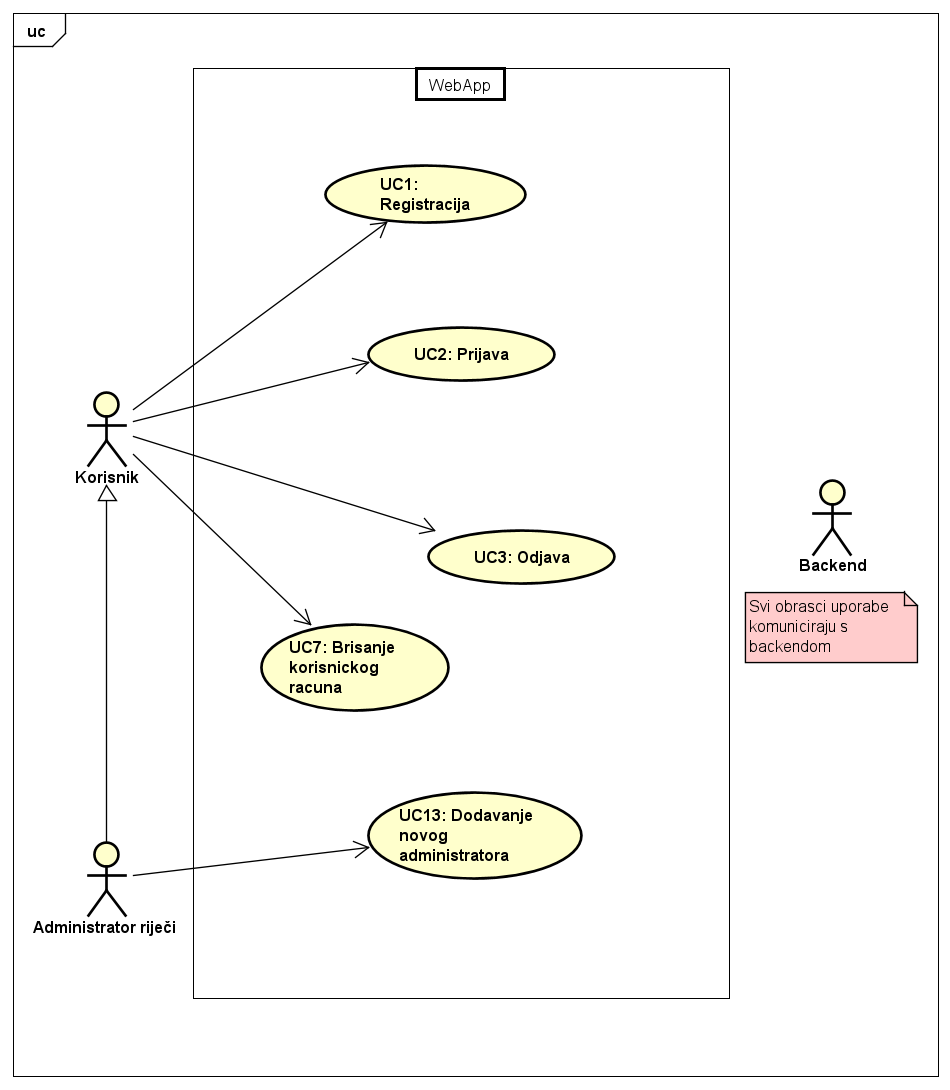
\includegraphics[width=\textwidth]{slike/UseCaseDiagram0.PNG}
						\caption{Dijagram obrazaca uporabe, funkcionalnosti korisnika i administratora riječi}
						\label{fig:useCaseDiagram0}
					\end{figure}
					
					\begin{figure}[H]
						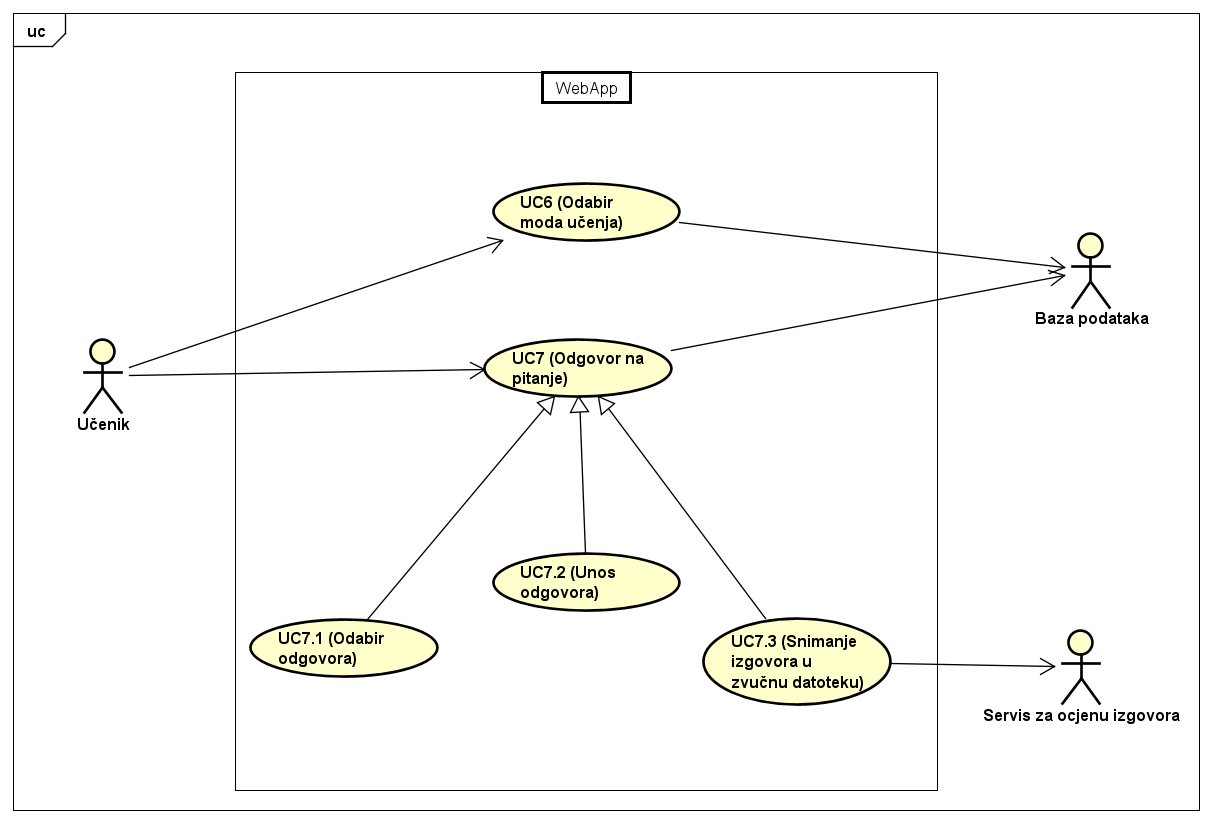
\includegraphics[width=\textwidth]{slike/UseCaseDiagram1.PNG}
						\caption{Dijagram obrazaca uporabe, funkcionalnosti korisnika}
						\label{fig:useCaseDiagram1}
					\end{figure}
					
					\begin{figure}[H]
						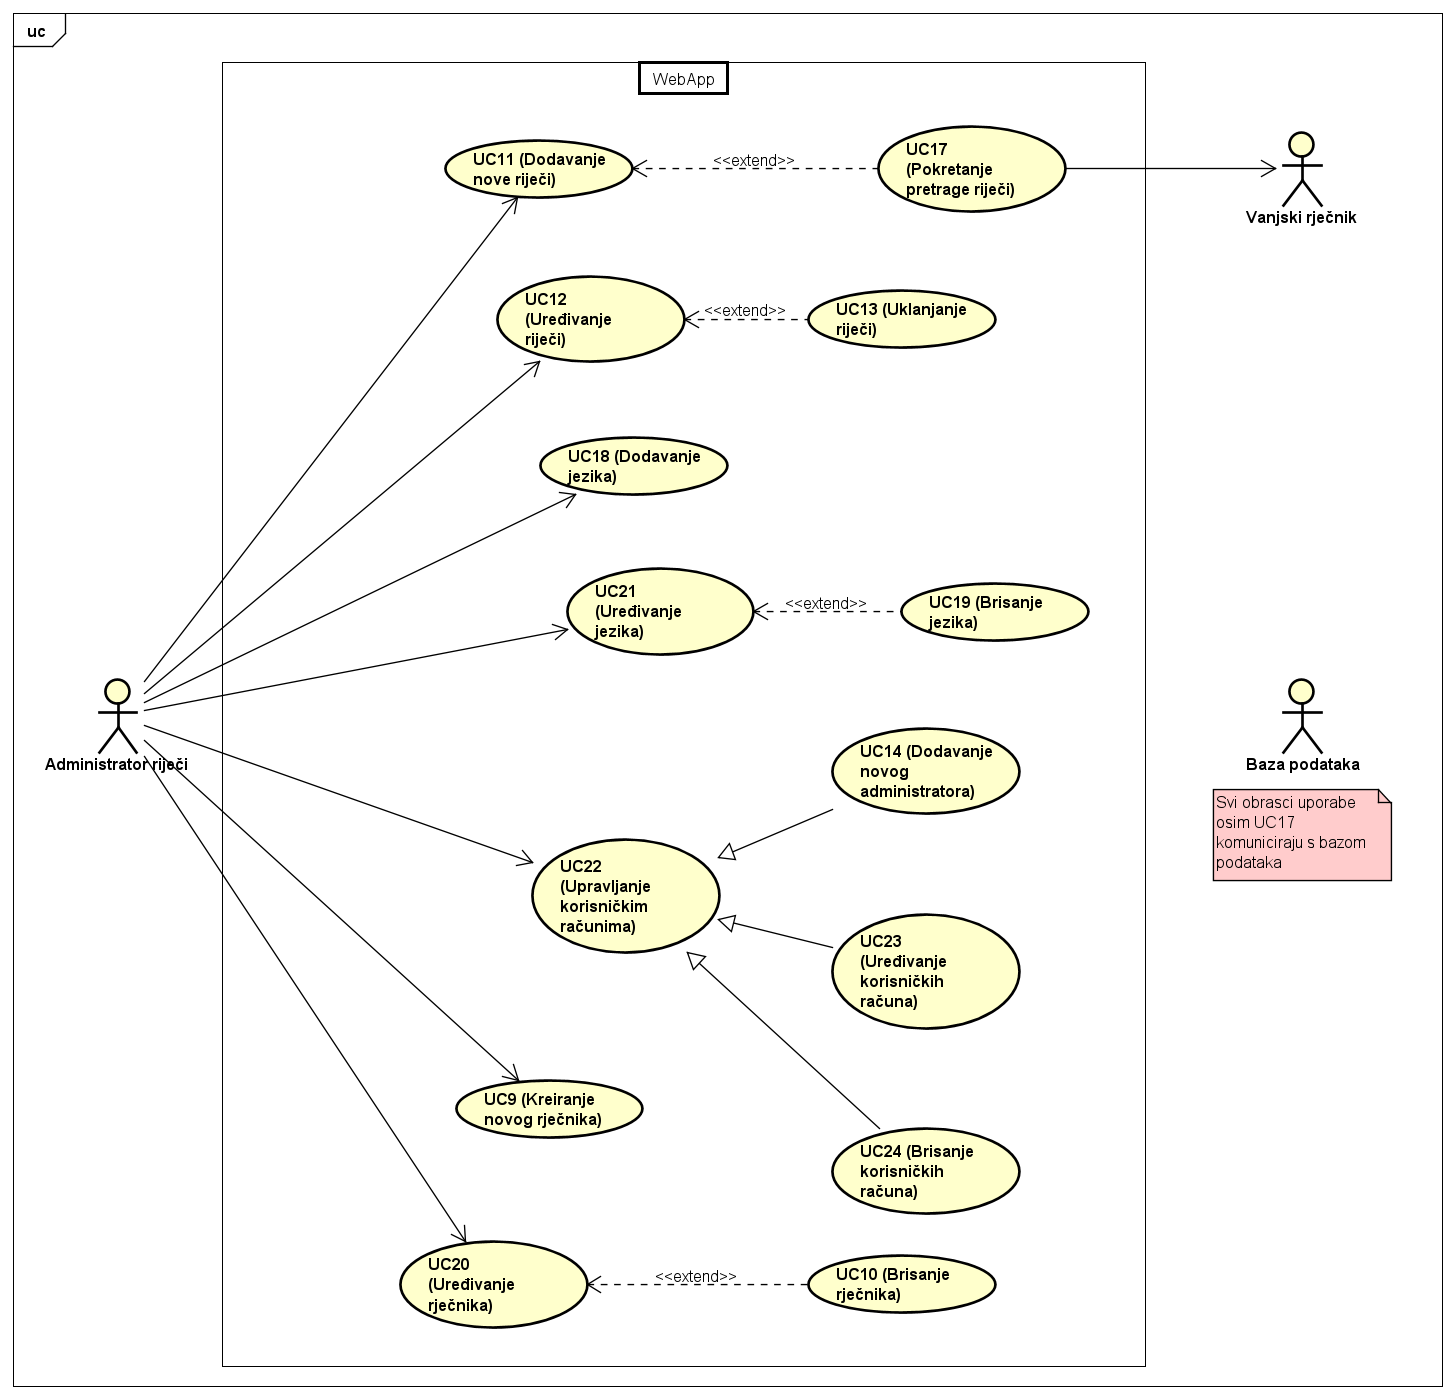
\includegraphics[width=\textwidth]{slike/UseCaseDiagram2.PNG}
						\caption{Dijagram obrazaca uporabe, funkcionalnosti administratora riječi}
						\label{fig:useCaseDiagram2}
					\end{figure} \newpage
				
			\subsection{Sekvencijski dijagrami}
				
%				\textbf{\textit{dio 1. revizije}}\\
%				
%				\textit{Nacrtati sekvencijske dijagrame koji modeliraju najvažnije dijelove sustava (max. 4 dijagrama). Ukoliko postoji nedoumica oko odabira, razjasniti s asistentom. Uz svaki dijagram napisati detaljni opis dijagrama.}
%				\eject
				
				\textbf{Obrazac uporabe UC1- Registracija}\\
				Korisnik odabire opciju „Registracija“. Sustav prikazuje formu za unos podataka za registraciju. Korisnik unosi potrebne podatke i potvrđuje registraciju.. Ako korisnik odustane od registracije, sustav vraća korisnika na početnu stranicu. Ako je korisnik unio mail adresu koja se već koristi u sustavu, sustav vraća obavijest o već registriranoj mail adresi. Ako mail adresa ne postoji u bazi podataka, sustav na navedenu mail adresu šalje mail s inicijalnom lozinkom.\newpage

				\begin{figure}[H]
					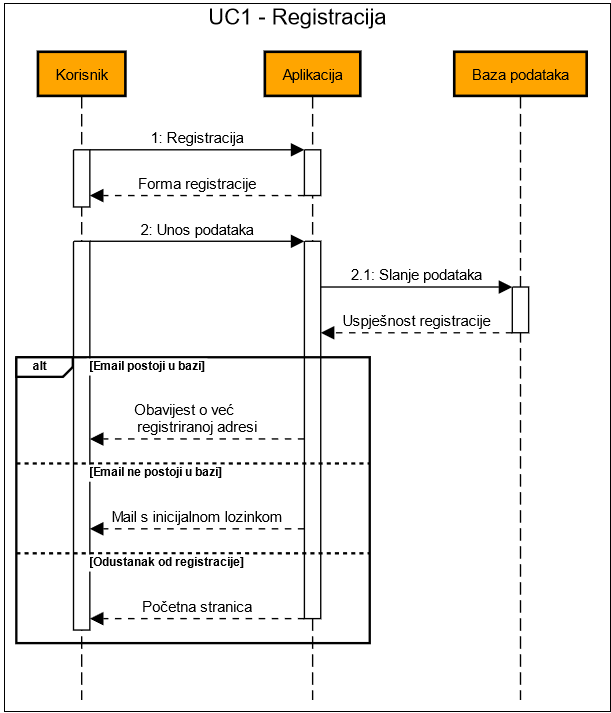
\includegraphics[width=\textwidth]{slike/UC1.PNG}
					\caption{Sekvencijski dijagram za UC1}
					\label{fig:sekv1}
				\end{figure} \newpage
				
				
				\noindent\textbf{Obrazac uporabe UC2 - Prijava}\\
				Korisnik odabire opciju „Prijava“. Sustav prikazuje formu za unos podataka za prijavu. Korisnik unosi potrebne podatke i potvrđuje prijavu. Sustav provjerava ispravnost podataka. Ako su podatci neispravni, sustav šalje obavijest o krivo unesenim podatcima, a korisnik mora ispraviti podatke i ponovno potvrditi prijavu sve dok ne budu uneseni ispravni podatci. Ako se korisnik po prvi puta prijavljuje u sustav, sustav mu prikazuje formu za promjenu inicijalne lozinke. Korisnik unosi novu lozinku, a sustav ju sprema u bazu podataka. Nakon prijave u sustav, sustav šalje korisnika na stranicu s ponuđenim jezicima.
				
				
				\begin{figure}[H]
					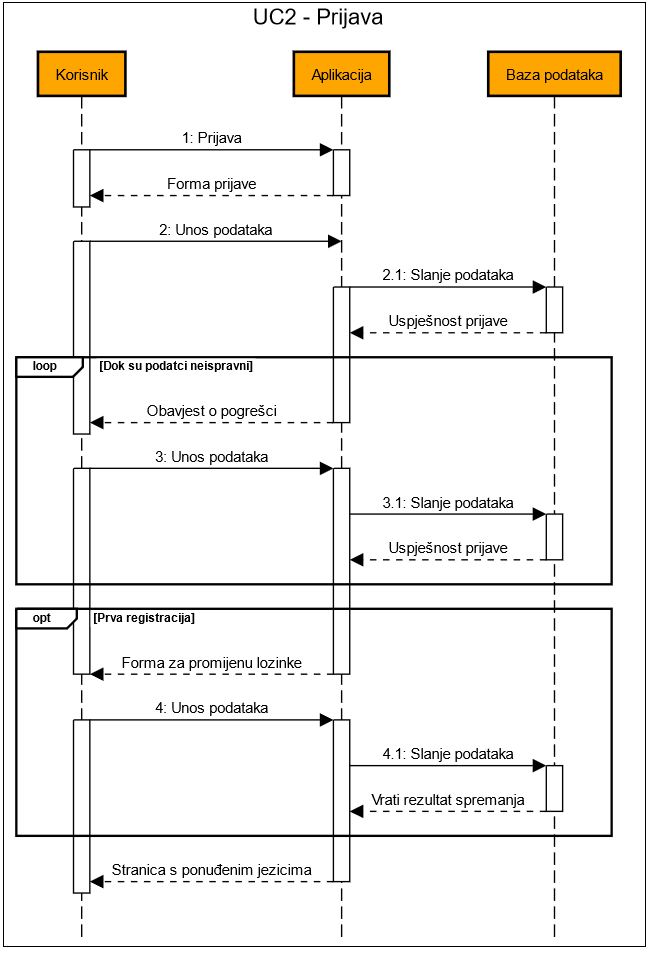
\includegraphics[width=\textwidth]{slike/UC2.PNG}
					\caption{Sekvencijski dijagram za UC2}
					\label{fig:sekv2}
				\end{figure} \newpage
								
				
				
				\noindent\textbf{Obrasci uporabe UC4, UC5 i UC6 - Odabir jezika, Odabir rječnika i moda učenja, Odgovor na pitanje}\\
				Korisnik odabire željeni jezik. Sustav iz baze podataka dohvaća rječnike koji su vezani za odabrani jezik te ih prikazuje korisniku. Korisnik odabire željeni rječnik. Sustav iz baze podataka dohvaća modove učenja te ih prikazuje korisniku. Korisnik odabire mod učenja. Sustav iz baze podataka dohvaća pitanje te prikazuje stranicu s pitanjem. Korisnik odgovara na pitanje te ako je odgovor točan, sustav u bazi podataka odgovoreno pitanje stavlja u iduću posudu. Ako je odgovor netočan, sustav u bazi podataka odgovoreno pitanje stavlja u prvu posudu. Korisnik odabire opciju „Sljedeće pitanje“. Sustav dohvaća novo pitanje iz baze podataka. Ako korisnik odustane od kviza, sustav ga vraća na stranicu s prikazom rječnika.
				
				\begin{figure}[H]
					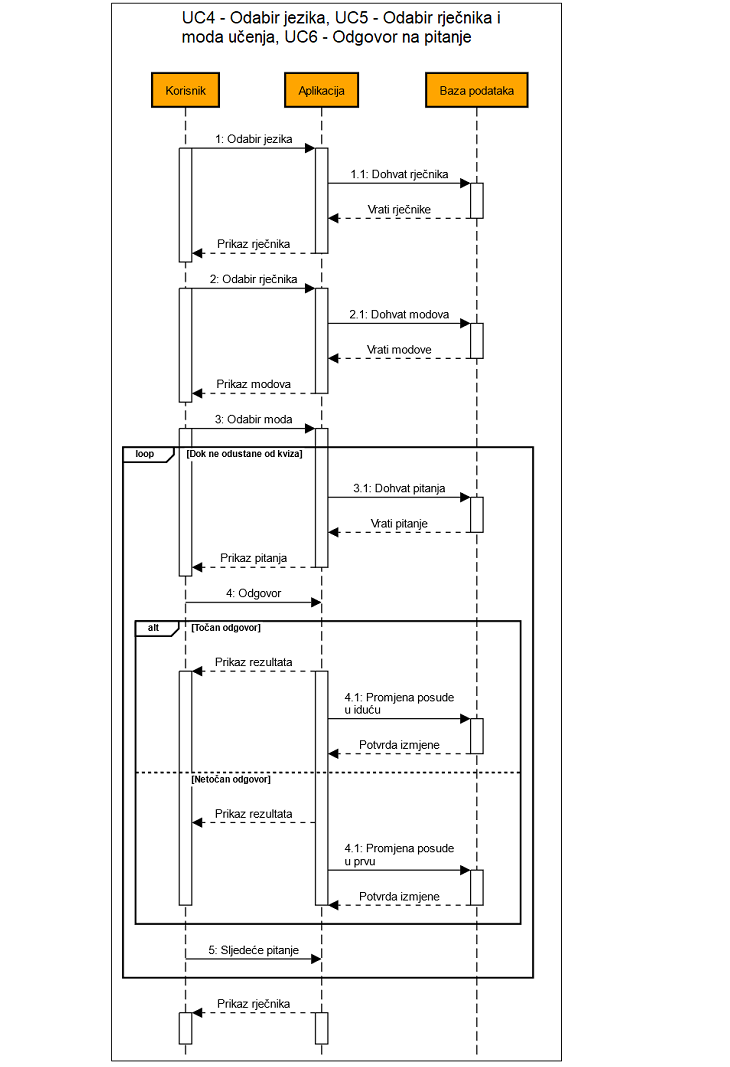
\includegraphics[width=\textwidth]{slike/UC4,UC5,UC6.PNG}
					\caption{Sekvencijski dijagram za UC4, UC5, UC6}
					\label{fig:sekv3}
				\end{figure} \newpage
				
				
				\noindent\textbf{Obrasci uporabe UC8 i UC10 - Kreiranje novog rječnika i Dodavanje nove riječi}\\
				Administrator odabire opciju „Kreiraj novi rječnik“. Sustav prikazuje formu za unos podataka novog rječnika. Administrator upisuje potrebne podatke. Ako su uneseni podatci neispravni, sustav prikazuje obavijest o neispravno unesenim podatcima, a administrator mora ispraviti unesene podatke. Kada su podatci ispravno uneseni, sustav podatke sprema u bazu podataka, a administratoru prikazuje početnu stranicu. Administrator odabire opciju „Dodaj novu riječ“. Sustav prikazuje formu za unos nove riječi. Nakon što administrator unese dio željene riječi, sustav pomoću vanjskih rječnika administratoru dojavljuje savjete s informacijama za unos riječi. Administrator odabire ponuđene riječi, upisuje potrebne podatke te odabire opciju „Spremi“. Sustav novu riječ sprema u bazu podataka, a administratora vraća na početnu stranicu.
				
				\begin{figure}[H]
					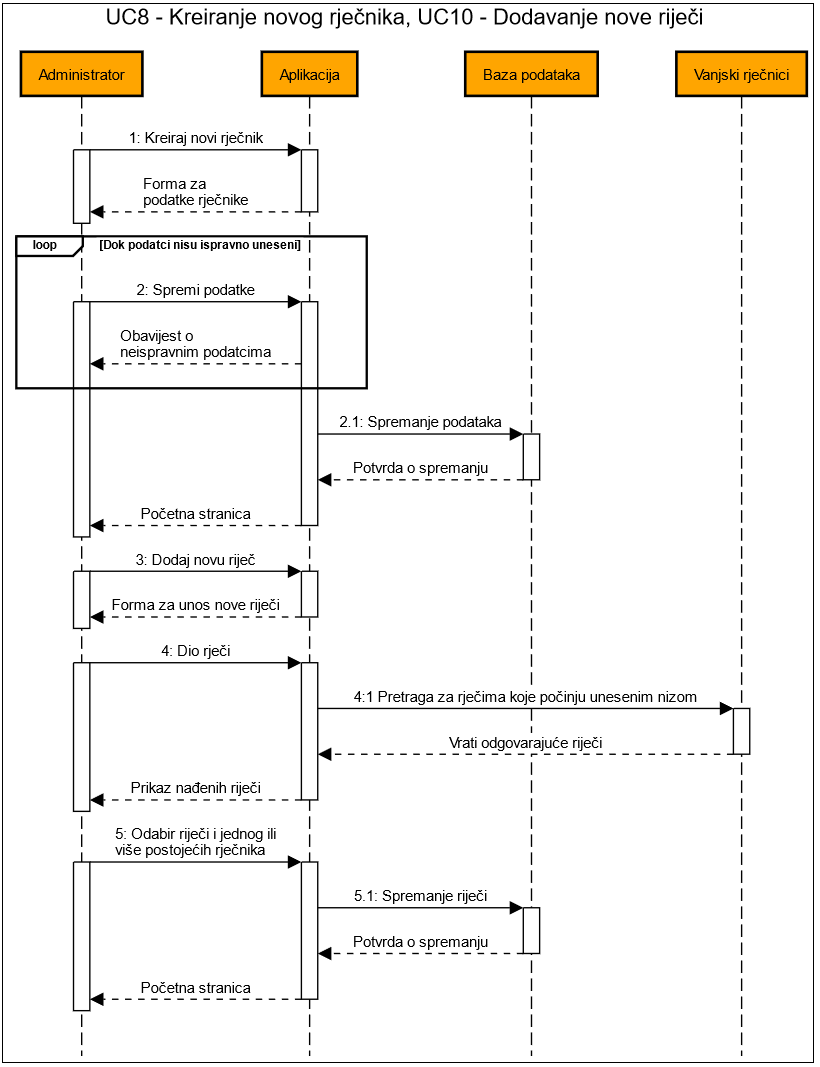
\includegraphics[width=\textwidth]{slike/UC8,UC10.PNG}
					\caption{Sekvencijski dijagram za UC8, UC10}
					\label{fig:sekv4}
				\end{figure} \newpage
	
		\section{Ostali zahtjevi}
		
			\begin{packed_enum}
				
				\item Sustav treba podržavati hrvatski jezik
				\item Sustav treba ostvariti kao web-aplikaciju
				\item Sustav treba koristiti vanjski API za dohvaćanje prijedloga riječi
				\item Sustavu se pristupa uz korištenje protokola HTTPS
				\item Sustav treba ostvariti pomoću objektno orijentiranog jezika
				\item Sve lozinke u sustavu trebaju biti kriptirane radi osiguravanja sigurnosti korisničkih računa
				\item Sustav treba ostvariti tako da bude jednostavan i intuitivan za korištenje
				\item Sustav treba moći pružati uslugu za više korisnika istovremeno
				
			\end{packed_enum}
		
%			\textbf{\textit{dio 1. revizije}}\\
%		 
%			 \textit{Nefunkcionalni zahtjevi i zahtjevi domene primjene dopunjuju funkcionalne zahtjeve. Oni opisuju \textbf{kako se sustav treba ponašati} i koja \textbf{ograničenja} treba poštivati (performanse, korisničko iskustvo, pouzdanost, standardi kvalitete, sigurnost...). Primjeri takvih zahtjeva u Vašem projektu mogu biti: podržani jezici korisničkog sučelja, vrijeme odziva, najveći mogući podržani broj korisnika, podržane web/mobilne platforme, razina zaštite (protokoli komunikacije, kriptiranje...)... Svaki takav zahtjev potrebno je navesti u jednoj ili dvije rečenice.}
			 
			 
			 
	
	\chapter{Arhitektura i dizajn sustava}
		
		%\textbf{\textit{dio 1. revizije}}\\

		%\textit{ Potrebno je opisati stil arhitekture te identificirati: podsustave, preslikavanje na radnu platformu, spremišta podataka, mrežne protokole, globalni upravljački tok i sklopovsko-programske zahtjeve. Po točkama razraditi i popratiti odgovarajućim skicama:}
	%\begin{itemize}
		%\item 	\textit{izbor arhitekture temeljem principa oblikovanja pokazanih na predavanjima (objasniti zašto ste baš odabrali takvu arhitekturu)}
		%\item 	\textit{organizaciju sustava s najviše razine apstrakcije (npr. klijent-poslužitelj, baza podataka, datotečni sustav, grafičko sučelje)}
		%\item 	\textit{organizaciju aplikacije (npr. slojevi frontend i backend, MVC arhitektura) }		
	%\end{itemize}

	
		Arhitektura sustava oblikovana je tako da se sastoji od tri podsustava:
		
		\begin{itemize}
			\item Web preglednik
			\item Web poslužitelj
			\item Baza podataka
		\end{itemize}
		
		\textbf{Web preglednik} služi korisniku za pristup poslužitelju i podacima u bazi podataka. To je program kojim korisnik može slati zahtjeve do poslužitelja za neku uslugu, u obliku dohvaćanja ili slanja podataka do poslužitelja. Web poslužitelj će nakon primitka zahtjeva od korisnika kroz Web preglednik prikazati odgovor na zahtjev. Dakle, Web preglednik je prvi korak za krajnjeg korisnika u interakciji sa sustavom u cjelini.
		
		
		\textbf{Web poslužitelj} je središnja komponenta sustava gdje se događaju svi važni izračuni te strukturiranje odgovora korisniku, a isto tako i pristup bazi podataka. To je program na jednom ili više računala, odnosno poslužitelja, koji interagira s jednim ili više korisnika. Zahtjeve prima preko HTTP protokola te vraća odgovor u obliku HTML dokumenta koji se prikazuje korisniku u njegovom Web pregledniku, potrebne podatke pohranjuje i ažurira u bazi podataka.
		
		
		\textbf{Baza podataka} je podsustav koji služi za pohranu svih potrebnih podataka. Backend strana Web aplikacije pristupa joj te upravlja podacima. Zbog učestalosti pristupa podacima u bazi podataka, od velike je važnosti da ona radi brzo i efikasno te je stoga bitno bazu podataka oblikovati efikasno i normalizirano.\\
		
		Arhitekturni stil koji je odabran za izradu sustava je model-pogled-nadglednik (engl. Model-View-Controller ili kraće MVC). MVC, ujedno i oblikovni obrazac, karakterizira njegova tri sloja model, view i controller.  
		
		\begin{itemize}
			\item \textbf{Model} je glavna komponenta ovog arhitekturnog stila. Sadrži razrede koji su vrlo slični tablicama u bazi podataka. Razredi modela opisuju strukture podataka te sadrže pravila i logiku rada aplikacije.
			\item \textbf{View} je komponenta koja se jedina ne nalazi na poslužiteljskoj strani. Ona služi za interakciju sustava s korisnikom, kako kroz zahtjeve korisnika, tako i kroz reprezentaciju odgovora poslužitelja krajnjem korisniku.
			\item \textbf{Controller} je komponenta koja upravlja zahtjevima krajnjeg korisnika na temelju modela. Također, ova komponenta upravlja odgovorima koji se dalje šalju do komponente View.
		\end{itemize}
		
		
		U izgradnji sustava koristi se objektno orijentirana paradigma. Za ovaj sustav to je programski jezik Java te radni okvir Spring koji je korišten za izradu backenda. Za izradu frontend dijela sustava, odnosno Web aplikacije upotrebljava se programski jezik JavaScript te biblioteka React. Uz to, za vanjsku komunikaciju kao pomoć u radu aplikacije, koristi se vanjski rječnik uz pomoć aplikacijskog sučelja.\\
		
		\newpage

				
		\section{Baza podataka}
			
			%\textbf{\textit{dio 1. revizije}}\\
			
		%\textit{Potrebno je opisati koju vrstu i implementaciju baze podataka ste odabrali, glavne komponente od kojih se sastoji i slično.}
		
\hspace*{6mm} Za potrebe rada sustava kojeg gradimo koristit ćemo relacijsku bazu podataka čiji su glavni elementi relacije. Relacije možemo promatrati kao tablice definirane svojim imenom te atributima. Relacijski model nastao je na temelju ER modela baze podataka čiji su temeljni elementi entiteti i veze. Zadatak baze podataka je brzo, kompaktno te jednostavno pohranjivanje, izmjenu te uklanjanje raznih podataka. Za ovaj sustav, to su podaci o korisničkim računima, podaci o pohranjenim rječnicima te riječima u njima, opisi riječi te stadij učenja u kojem se nalazi korisnik sustava. U skladu s tim, definiramo bazu podataka sastavljenu od entiteta:
			
			\begin{packed_item}
				
				\item Account
				\item AccountType
				\item CurrentState
				\item Pot
				\item LearningMode
				\item Dictionary
				\item Language
				\item Phrase
				\item Word
				\item wordInDict
				\item wordInPot
				
			\end{packed_item}
		
			\subsection{Opis tablica}
			

%				\textit{Svaku tablicu je potrebno opisati po zadanom predlošku. Lijevo se nalazi točno ime varijable u bazi podataka, u sredini se nalazi tip podataka, a desno se nalazi opis varijable. Svjetlozelenom bojom označite primarni ključ. Svjetlo plavom označite strani ključ}
				
				
				\hspace*{6mm} \textbf{Account} Ovaj entitet sadrži informacije o korisničkom računu. Njegovi atributi su: accountID, accountEmail, personName, personSurname, accountPassword te accountTypeID. Ovaj entitet u vezi \textit{Many-to-One} je s entitetom AccountType preko atributa accountTypeID, u vezi \textit{One-to-Many} s entitetom Pot preko atributa accountID te u vezi \textit{One-to-Many} s entitetom CurrentState preko atributa accountID.
				
				\begin{longtblr}[
					label=racun,
					entry=none
					]{
						width = \textwidth,
						colspec={|X[8,l]|X[6, l]|X[18, l]|}, 
						rowhead = 1,
					} %definicija širine tablice, širine stupaca, poravnanje i broja redaka naslova tablice
					\hline \SetCell[c=3]{c}{\textbf{Account}}	 \\ \hline[3pt]
					\SetCell{LightGreen}accountID & INT	&  	Jedinstven identifikator korisnika generiran od strane baze podataka (surogatni ključ)  	\\ \hline
					accountEmail	& VARCHAR &   Jedinstvena adresa elektroničke pošte (alternativni ključ)	\\ \hline 
					personName & VARCHAR & Ime korisnika  \\ \hline 
					personSurname & VARCHAR	&  	Prezime korisnika	\\ \hline 
					accountPassword & VARCHAR & Kriptirana lozinka korisnika  \\ \hline
					\SetCell{LightBlue} accountTypeID	& INT &   Identifikator vrste računa korisnika	\\ \hline 
				\end{longtblr}
				
				\textbf{AccountType} Ovaj entitet sadrži informacije o vrsti korisničkog računa (radi li se o učeniku ili administratoru riječi). Njegovi atributi su: accountTypeID te accountTypeName. Ovaj entitet u vezi \textit{One-to-Many} je s entitetom Account preko atributa accountTypeID.
				
				\begin{longtblr}[
					label=vrstaRacuna,
					entry=none
					]{
						width = \textwidth,
						colspec={|X[8,l]|X[6, l]|X[18, l]|}, 
						rowhead = 1,
					} %definicija širine tablice, širine stupaca, poravnanje i broja redaka naslova tablice
					\hline \SetCell[c=3]{c}{\textbf{AccountType}}	 \\ \hline[3pt]
					\SetCell{LightGreen}accountTypeID & INT	&  Jedinstven identifikator vrste računa generiran od strane baze podataka (surogatni ključ)  	\\ \hline
					accountTypeName	& VARCHAR &   Ime vrste računa	\\ \hline  
				\end{longtblr}
				
				\textbf{CurrentState} Ovaj slabi entitet sadrži informacije o trenutnom stanju u kojem se nalazi korisnik sustava. Njegovi atributi su: dictionaryID, accountID, learningModeID. Ovaj entitet u vezi \textit{Many-to-One} je s entitetom Dictionary preko atributa dictionaryID, u vezi \textit{Many-to-One} je s entitetom Account preko atributa accountID, u vezi \textit{Many-to-One} je s entitetom LearningMode preko atributa learningModeID.
				
				\begin{longtblr}[
					label=trenutnoStanje,
					entry=none
					]{
						width = \textwidth,
						colspec={|X[8,l]|X[6, l]|X[18, l]|}, 
						rowhead = 1,
					} %definicija širine tablice, širine stupaca, poravnanje i broja redaka naslova tablice
					\hline \SetCell[c=3]{c}{\textbf{CurrentState}}	 \\ \hline[3pt]
					\SetCell{LightGreen}dictionaryID & INT	&  	Jedinstven identifikator rječnika (strani ključ)	\\ \hline
					\SetCell{LightGreen}accountID & INT	&  	Jedinstven identifikator računa (strani ključ)	\\ \hline
					\SetCell{LightGreen}learningModeID & INT	&  	Jedinstven identifikator moda (strani ključ) učenja 	\\ \hline
				\end{longtblr}
				
				\textbf{Pot} Ovaj slabi entitet sadrži informacije o pojedinoj posudi riječi pridruženoj nekom korisniku. Njegovi atributi su: potID, accountID, expirationTime, potNumber. Ovaj entitet u vezi \textit{Many-to-One} je s entitetom Account preko atributa accountID, u vezi \textit{Many-to-Many} je s entitetom Word preko atributa wordID, potID, accountID.
				
				\begin{longtblr}[
					label=posuda,
					entry=none
					]{
						width = \textwidth,
						colspec={|X[7,l]|X[6, l]|X[19, l]|}, 
						rowhead = 1,
					} %definicija širine tablice, širine stupaca, poravnanje i broja redaka naslova tablice
					\hline \SetCell[c=3]{c}{\textbf{Pot}}	 \\ \hline[3pt]
					\SetCell{LightGreen}potID & INT	&  Jedinstveni identifikator posude riječi 	\\ \hline
					\SetCell{LightGreen}accountID & INT & Jedinstveni identifikator računa korisnika (strani ključ) \\ \hline
					expirationTime & INTERVAL & Vrijeme koje je potrebno proći kako bi se riječi iz posude pojavile u pitanju korisniku  \\ \hline 
					potNumber & INT	&  	Redni broj posude (alternativni ključ)	\\ \hline 
				\end{longtblr}
				
				\textbf{LearningMode} Ovaj entitet sadrži informacije o modu učenja u kojem je korisnik. Njegovi atributi su: learningModeID, learningModeDescription. Ovaj entitet u vezi \textit{One-to-Many} je s entitetom CurrentState preko atributa learningModeID. \newpage
				
				\begin{longtblr}[
					label=modUcenja,
					entry=none
					]{
						width = \textwidth,
						colspec={|X[11,l]|X[6, l]|X[15, l]|}, 
						rowhead = 1,
					} %definicija širine tablice, širine stupaca, poravnanje i broja redaka naslova tablice
					\hline \SetCell[c=3]{c}{\textbf{LearningMode}}	 \\ \hline[3pt]
					\SetCell{LightGreen}learningModeID & INT	&  Jedinstven identifikator moda učenja generiran od strane baze podataka (surogatni ključ)  	\\ \hline
					learningModeDescription	& VARCHAR &   Kratki opis moda učenja	\\ \hline 
				\end{longtblr}
				
				\textbf{Dictionary} Ovaj entitet sadrži informacije o rječniku za neki jezik. Njegovi atributi su: dictionaryID, dictionaryName, languageID. Ovaj entitet u vezi \textit{One-to-Many} je s entitetom CurrentState preko atributa dictionaryID, u vezi \textit{Many-to-One} s entitetom Language preko atributa languageID te u vezi \textit{Many-to-Many} s entitetom Word preko atributa dictionaryID, wordID.
				
				\begin{longtblr}[
					label=rjecnik,
					entry=none
					]{
						width = \textwidth,
						colspec={|X[7,l]|X[6, l]|X[19, l]|}, 
						rowhead = 1,
					} %definicija širine tablice, širine stupaca, poravnanje i broja redaka naslova tablice
					\hline \SetCell[c=3]{c}{\textbf{Dictionary}}	 \\ \hline[3pt]
					\SetCell{LightGreen}dictionaryID & INT	&  	Jedinstveni identifikator rječnika generiran od strane baze podataka (surogatni ključ)  	\\ \hline
					dictionaryName	& VARCHAR &   Ime rječnika	\\ \hline 
					\SetCell{LightBlue}languageID	& INT &   Jedinstveni identifikator jezika kojem je rječnik pridružen	\\ \hline 
				\end{longtblr}
				
				\textbf{Language} Ovaj entitet sadrži informacije o jeziku kojeg podržava sustav. Njegovi atributi su: languageID, languageCode, languageName. Ovaj entitet u vezi \textit{One-to-Many} je s entitetom Dictionary preko atributa languageID.
				
				\begin{longtblr}[
					label=jezik,
					entry=none
					]{
						width = \textwidth,
						colspec={|X[6,l]|X[6, l]|X[20, l]|}, 
						rowhead = 1,
					} %definicija širine tablice, širine stupaca, poravnanje i broja redaka naslova tablice
					\hline \SetCell[c=3]{c}{\textbf{Language}}	 \\ \hline[3pt]
					\SetCell{LightGreen}languageID & INT	&  Jedinstveni identifikator jezika generiran od strane baze podataka (surogatni ključ)	\\ \hline
					languageCode	& CHAR &   Troslovna kratica jezika	\\ \hline 
					languageName & VARCHAR & Ime jezika  \\ \hline 
				\end{longtblr}
				
				\textbf{Phrase} Ovaj entitet sadrži informacije o frazi koja bolje opisuje neku riječ. Njegovi atributi su: phraseID, phraseContent, wordID. Ovaj entitet u vezi \textit{Many-to-One} je s entitetom Word preko atributa wordID.
				
				\begin{longtblr}[
					label=fraza,
					entry=none
					]{
						width = \textwidth,
						colspec={|X[6,l]|X[6, l]|X[20, l]|}, 
						rowhead = 1,
					} %definicija širine tablice, širine stupaca, poravnanje i broja redaka naslova tablice
					\hline \SetCell[c=3]{c}{\textbf{Phrase}}	 \\ \hline[3pt]
					\SetCell{LightGreen}phraseID & INT	&  	Jedinstveni identifikator fraze generiran od strane baze podataka (surogatni ključ)  	\\ \hline
					phraseContent	& VARCHAR &   Tekst fraze	\\ \hline 
					\SetCell{LightBlue}wordID	& INT &   Jedinstveni identifikator riječi kojoj je fraza pridružena	\\ \hline 
				\end{longtblr}
				
				\textbf{Word} Ovaj entitet sadrži informacije o riječi koja je dodana u sustav. Njegovi atributi su: wordID, wordContent, wordPronunciation. Ovaj entitet u vezi \textit{Many-to-Many} je s entitetom Pot preko atributa potID, wordID, accountID, u vezi \textit{Many-to-One} s entitetom Phrase preko atributa phraseID, u vezi je \textit{Many-to-Many} s entitetom Dictionary preko atributa dictionaryID, wordID.
				
				\begin{longtblr}[
					label=rijec,
					entry=none
					]{
						width = \textwidth,
						colspec={|X[9,l]|X[6, l]|X[17, l]|}, 
						rowhead = 1,
					} %definicija širine tablice, širine stupaca, poravnanje i broja redaka naslova tablice
					\hline \SetCell[c=3]{c}{\textbf{Word}}	 \\ \hline[3pt]
					\SetCell{LightGreen}wordID & INT	&  Jedinstveni identifikator riječi generiran od strane baze podataka (surogatni ključ)	\\ \hline
					wordContent	& VARCHAR &   Sadržaj riječi	\\ \hline 
					wordPronunciation & BYTEA & Glasovna datoteka koja predstavlja izgovor riječi  \\ \hline 
				\end{longtblr}
				
				\textbf{wordInDict} Ovaj entitet nastao zbog veze \textit{Many-to-Many} sadrži informacije o tome u kojim rječnicima se nalazi riječ. Njegovi atributi su: wordID, dictionaryID.
				
				\begin{longtblr}[
					label=rijecURjecniku,
					entry=none
					]{
						width = \textwidth,
						colspec={|X[6,l]|X[6, l]|X[20, l]|}, 
						rowhead = 1,
					} %definicija širine tablice, širine stupaca, poravnanje i broja redaka naslova tablice
					\hline \SetCell[c=3]{c}{\textbf{wordInDict}}	 \\ \hline[3pt]
					\SetCell{LightGreen}dictionaryID & INT	&  	Jedinstven identifikator rječnika (strani ključ)	\\ \hline
					\SetCell{LightGreen}wordID & INT	&  	Jedinstven identifikator riječi (strani ključ)	\\ \hline
				\end{longtblr}
				
				\textbf{wordInPot} Ovaj entitet nastao zbog veze \textit{Many-to-Many} sadrži informacije o u kojoj se posudi za koji račun nalazi neka riječ. Njegovi atributi su: wordID, potID, accountID.
				
				\begin{longtblr}[
					label=rijecUPosudi,
					entry=none
					]{
						width = \textwidth,
						colspec={|X[6,l]|X[6, l]|X[20, l]|}, 
						rowhead = 1,
					} %definicija širine tablice, širine stupaca, poravnanje i broja redaka naslova tablice
					\hline \SetCell[c=3]{c}{\textbf{wordInPot}}	 \\ \hline[3pt]
					\SetCell{LightGreen}wordID & INT	&  	Jedinstven identifikator riječi (strani ključ)	\\ \hline
					\SetCell{LightGreen}accountID & INT	&  	Jedinstven identifikator računa (strani ključ)	\\ \hline
					\SetCell{LightGreen}potID & INT	&  	Jedinstven identifikator posude (strani ključ) učenja 	\\ \hline 
				\end{longtblr}
				
				
			
			\subsection{Dijagram baze podataka}
%				\textit{ U ovom potpoglavlju potrebno je umetnuti dijagram baze podataka. Primarni i strani ključevi moraju biti označeni, a tablice povezane. Bazu podataka je potrebno normalizirati. Podsjetite se kolegija "Baze podataka".}
			
%			\eject

				\begin{figure}[H]
					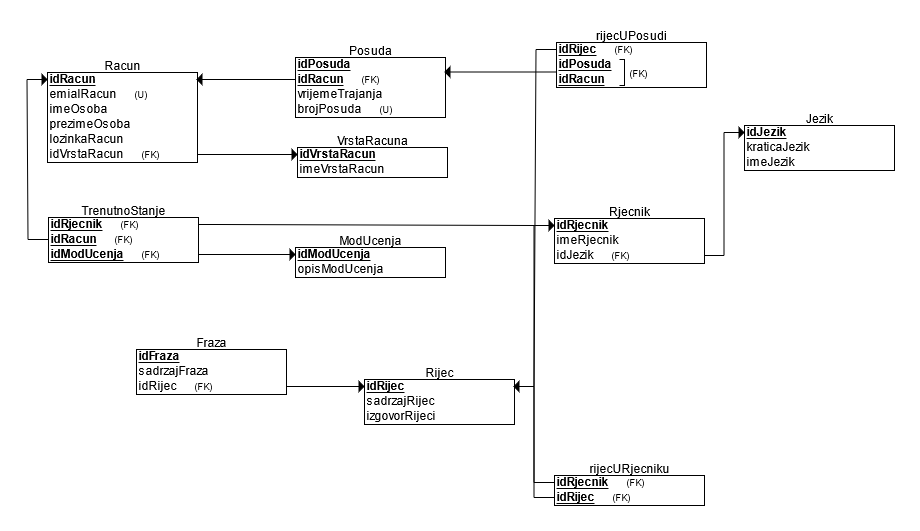
\includegraphics[width=\textwidth]{slike/dijagramBP.PNG}
					\caption{Dijagram baze podataka}
					\label{fig:dijagramBP}
				\end{figure}
				
				\newpage
			
			
		\section{Dijagram razreda}
		
			%\textit{Potrebno je priložiti dijagram razreda s pripadajućim opisom. Zbog preglednosti je moguće dijagram razlomiti na više njih, ali moraju biti grupirani prema sličnim razinama apstrakcije i srodnim funkcionalnostima.}\\
			
			%\textbf{\textit{dio 1. revizije}}\\
			
			%\textit{Prilikom prve predaje projekta, potrebno je priložiti potpuno razrađen dijagram razreda vezan uz \textbf{generičku funkcionalnost} sustava. Ostale funkcionalnosti trebaju biti idejno razrađene u dijagramu sa sljedećim komponentama: nazivi razreda, nazivi metoda i vrste pristupa metodama (npr. javni, zaštićeni), nazivi atributa razreda, veze i odnosi između razreda.}\\
			
			\begin{figure}[H]
				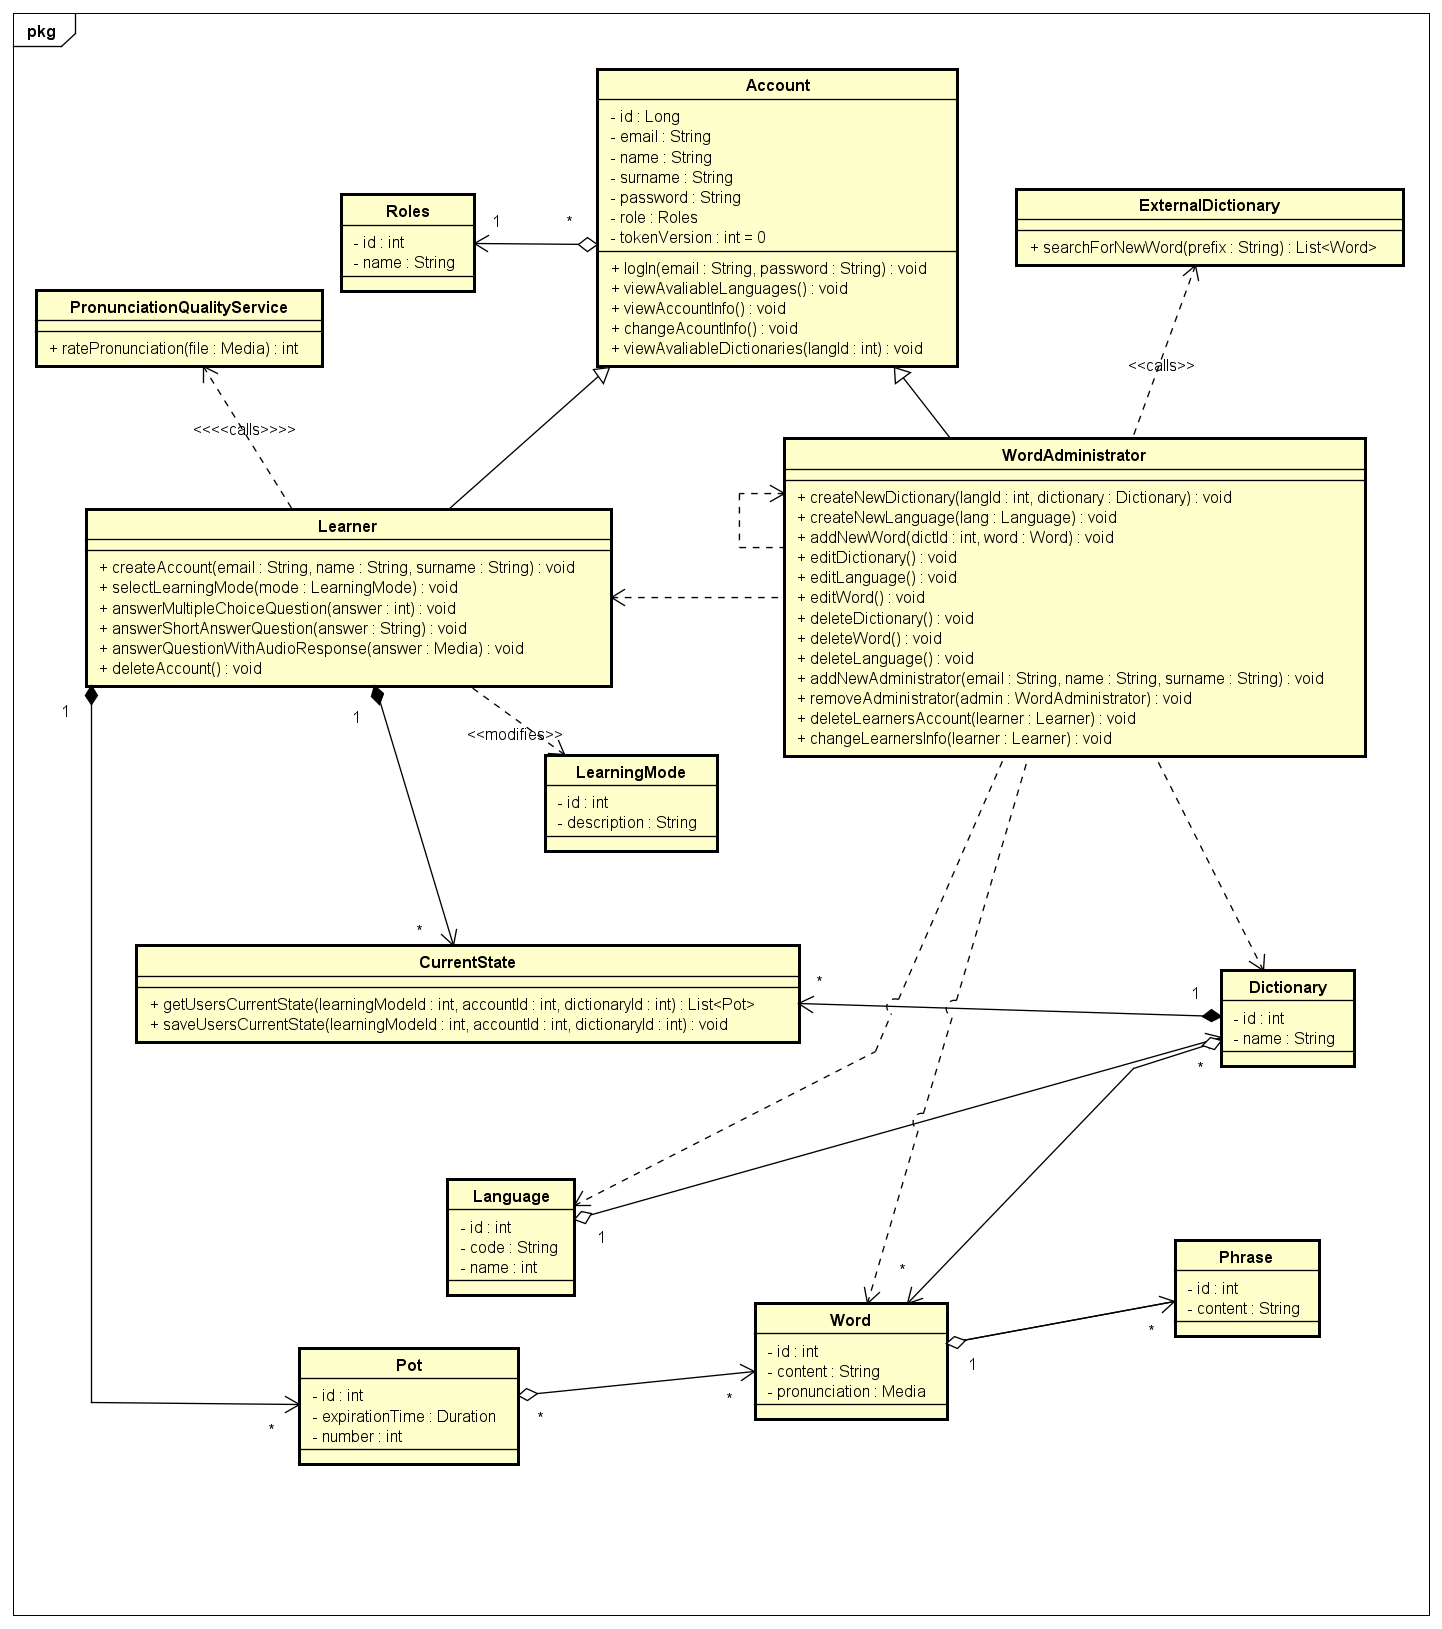
\includegraphics[width=\textwidth]{slike/ClassDiagram1.PNG}
				\caption{Dijagram razreda - modeli}
				\label{fig:classDiagram1}
			\end{figure}
			
			\newpage
			
			Slika 4.2 prikazuje razrede koji predstavljaju model u arhitekturi sustava. Dijagram je idejno razrađen. Čini ga razred Roles kojim označavamo o kojem se tipu korisničkog računa radi. On je vezan uz razred Account koji označava sam korisnički račun. Kako postoji više vrsta korisničkog računa te kako sve funkcionalnosti nisu iste za sve vrste korisničkih računa, postoje i razredi Learner i WordAdministrator koji su izvedene razreda Account razreda. Za razred WordAdministrator postoji rekurzivna ovisnost jer je moguće kreirati nove administratore riječi ako je korisnik također administrator riječi. Uz razred Learner veže se razred PronunciationQualityService koji je servis za ocjenu kvalitete izgovora riječi ako je učenik u tom modu učenja, razred LearningMode koji predstavlja mod učenja te ga učenik može promijeniti. Uz razred Learner također se veže i razred CurrentState koji označava trenutno stanje u kojem se učenik nalazi za prije odabrani rječnik. Nadalje, uz razred CurrentState veže se i razred Dictionary koji predstavlja rječnik. Uz rječnik je povezan razred Language jer rječnik pripada jeziku. Uz rječnik također je povezan i razred Word koji predstavlja riječ. Riječ je bolje opisana s nekoliko fraza koje su u modelu sustava razred Phrase. Uz razrede Learner i Word veže se i razred Pot koji je model posude u koju su spremljene riječi i to različito za svakog korisnika. Razredi Language, Word i Dictionary vezani su uz razred WordAdministrator jer administrator riječi može dodavati, brisati i mijenjati sadržaj jezika, rječnika i riječi. Na kraju, postoji i razred ExternalDictionary koji administrator riječi poziva ako želi dobiti prijedlog riječi koje zatim može dodati u neki od rječnika u sustavu. \newpage
			
			\begin{figure}[H]
				\includegraphics[width=\textwidth]{slike/ClassDiagram0.PNG}
				\caption{Dijagram razreda - generičke funkcionalnosti}
				\label{fig:classDiagram0}
			\end{figure}
			
			\newpage
			
			Slika 4.3 prikazuje detaljnije razrađen dijagram razreda, ali samo za generičke funkcionalnosti. Razred Account predstavlja istoimeni entitet u bazi podataka s brojnim metodama. On je povezan s enumeracijskim razredom Roles koji predstavlja listu svih mogućih vrsta korisničkog računa. Na dijagramu su također prikazana i dva kontrolera. AuthenticationController provjerava i odgovara na zahtjeve za ulazak u sustav i izlazak iz istoga. AccountController služi za promjenu podataka u sustavu za korisnički račun te također služi i uklanjanje računa iz sustava. Sučelje AccountService, razredi AccountServiceJpa kao njegova implementacija te AccountUserDetailsService služe za manipulaciju s korisničkim računima kroz bazu podataka. Slično, sučelje AuthenticationService i razred AuthenticationServiceJpa kao implementacija sučelja služe da ulazak u sustav te provjeru ispravnosti podataka kojima korisnik želi pristupiti sustavu. Uz to, postoje i neke sigurnosne klase koje služe za očuvanje sigurnosti podataka i sustava.
			
			\newpage
			
			\textbf{\textit{dio 2. revizije}}\\			
			
			\textit{Prilikom druge predaje projekta dijagram razreda i opisi moraju odgovarati stvarnom stanju implementacije}
			
			
			
			\eject
		
		\section{Dijagram stanja}
			
			
			\textbf{\textit{dio 2. revizije}}\\
			
			\textit{Potrebno je priložiti dijagram stanja i opisati ga. Dovoljan je jedan dijagram stanja koji prikazuje \textbf{značajan dio funkcionalnosti} sustava. Na primjer, stanja korisničkog sučelja i tijek korištenja neke ključne funkcionalnosti jesu značajan dio sustava, a registracija i prijava nisu. }
			
			
			\eject 
		
		\section{Dijagram aktivnosti}
			
			\textbf{\textit{dio 2. revizije}}\\
			
			 \textit{Potrebno je priložiti dijagram aktivnosti s pripadajućim opisom. Dijagram aktivnosti treba prikazivati značajan dio sustava.}
			
			\eject
		\section{Dijagram komponenti}
		
			\textbf{\textit{dio 2. revizije}}\\
		
			 \textit{Potrebno je priložiti dijagram komponenti s pripadajućim opisom. Dijagram komponenti treba prikazivati strukturu cijele aplikacije.}
	\chapter{Implementacija i korisničko sučelje}
		
		
		\section{Korištene tehnologije i alati}
		
			%\textbf{\textit{dio 2. revizije}}
			
			 %\textit{Detaljno navesti sve tehnologije i alate koji su primijenjeni pri izradi dokumentacije i aplikacije. Ukratko ih opisati, te navesti njihovo značenje i mjesto primjene. Za svaki navedeni alat i tehnologiju je potrebno \textbf{navesti internet poveznicu} gdje se mogu preuzeti ili više saznati o njima}.
			 
			 Za ostvarenje komunikacije između članova projektnog tima korištena je aplikacija WhatsApp\footnote{\url{https://www.whatsapp.com/}}. Za održavanje sastanaka unutar tima korištena je platforma MS Teams\footnote{\url{https://www.microsoft.com/microsoft-teams/}}. Komunikacija s demonstratorom i asistentom ostvarena je također s pomoću platforme MS Teams. Praćenje napretka i raspodjela zadataka u timu ostvarena je pomoću alata Jira\footnote{\url{https://www.atlassian.com/software/jira}}. Jira pomoću tzv. issue nudi pogućnost podijele izrade u manje zadatke koji se zatim mogu pridijeliti nekom od članova tima. Svaki od člana tima zatim može za svaki zadatak prikazati u kojoj je fazi izrade što ostalim članovima nudi mogućnost uvida u to na čemu drugi članovi tima trenutno rade. Upravljanje izvornim kodom i dokumentacijom ostvareno je s pomoću alata Git\footnote{\url{https://git-scm.com/}}. Udaljeni repozitorij pohranjen je na platformi GitHub\footnote{\url{https://github.com/}}. Za izradu dokumentacije projekta korišten je LaTeX\footnote{\url{https://www.latex-project.org/}}. UML dijagram obrazaca uporabe, sekvencijski dijagram, prva revizija dijagrama razreda, dijagram aktivnosti, dijagram stanja, dijagram komponenti i dijagram razmještaja napravljeni su s pomoću alata Astah UML\footnote{\url{https://astah.net/products/astah-uml/}}. Implementacijski dijagram razreda napravljen je s pomoću alata IntelliJ IDEA\footnote{\url{https://www.jetbrains.com/idea/}}. Model baze podataka izgrađen je alatom ERDPlus\footnote{\url{https://erdplus.com/}}. Za izradu backend dijela aplikacije korišten je radni okvir Java\footnote{\url{https://www.java.com/en/}} Spring\footnote{\url{https://spring.io/}}, a za razvoj na backendu korišteno je razvojno okruženje IntelliJ IDEA. Za izradu frontend dijela aplikacije korištena je knjižnica React\footnote{\url{https://react.dev/}} uz programski jezik TypeScript\footnote{\url{https://www.typescriptlang.org/}}. Za ispitivanje sustava korišteni su JUnit\footnote{\url{https://junit.org/}} i Selenium\footnote{\url{https://www.selenium.dev/}}. Za puštanje aplikacije u pogon korištena je platforma Render\footnote{\url{https://render.com/}}.
			
			
			\eject 
		
	
		\section{Ispitivanje programskog rješenja}

			\subsection{Ispitivanje komponenti}
			
			\subsubsection{Testiranje Gettera i Settera}
			
			TestGettersAndSetters služi za provjeru ispravnosti gettera i settera za klasu \texttt{Account}. U ovom testu se inicijalizira objekt \texttt{Account} s određenim podacima (email, ime, prezime, lozinka, i uloga), a zatim se koriste getteri za dohvaćanje tih podataka i setteri za postavljanje novih vrijednosti. Nakon postavljanja novih vrijednosti, ponovno se koriste getteri za provjeru je li objekt uspješno promijenjen prema očekivanjima.
			
			\begin{lstlisting}[language=Java]
@Test
public void testGettersAndSetters() {
	Account account = new Account("test@example.com", "John", 
				"Doe", "password", Roles.USER);
	
	Assertions.assertEquals("test@example.com", 
				account.getEmail());
	Assertions.assertEquals("John", account.getFirstName());
	Assertions.assertEquals("Doe", account.getLastName());
	Assertions.assertEquals("password", account.getPassword());
	Assertions.assertEquals(Roles.USER, account.getRole());
	
	account.setEmail("newemail@example.com");
	account.setFirstName("Jane");
	account.setLastName("Smith");
	account.setPassword("newpassword");
	account.setRole(Roles.ADMIN);
	
	Assertions.assertEquals("newemail@example.com", 
				account.getEmail());
	Assertions.assertEquals("Jane", account.getFirstName());
	Assertions.assertEquals("Smith", account.getLastName());
	Assertions.assertEquals("newpassword", account.getPassword());
	Assertions.assertEquals(Roles.ADMIN, account.getRole());
}
			\end{lstlisting}
			
			\subsubsection{Testiranje Token Verzije}
			
			TestTokenVersion provjerava funkcionalnost metoda za rad s token verzijom \\(\texttt{getTokenVersion()}, \texttt{incrementTokenVersion()}, \texttt{setTokenVersion()}) za klasu \texttt{Account}. Prvo se inicijalizira objekt \texttt{Account}, a zatim se provjerava da li je početna vrijednost token verzije jednaka 0. Nakon toga, koristi se metoda \texttt{incrementTokenVersion()} za povećanje verzije za 1 i provjerava se da li je nova vrijednost 1. Također se koristi metoda \texttt{setTokenVersion()} za postavljanje verzije na 5 i provjerava se je li postavljena vrijednost ispravna.
			
			\begin{lstlisting}[language=Java]
@Test
public void testTokenVersion() {
	Account account = new Account("test@example.com", "John", 
				"Doe", "password", Roles.USER);
	
	Assertions.assertEquals(0L, account.getTokenVersion());
	
	account.incrementTokenVersion();
	Assertions.assertEquals(1L, account.getTokenVersion());
	
	account.setTokenVersion(5L);
	Assertions.assertEquals(5L, account.getTokenVersion());
}
			\end{lstlisting}
			
			\subsubsection{Testiranje Metode \texttt{toString()}}
			
			ToString test provjerava da li metoda \texttt{toString()} klase \texttt{Account} vraća očekivani format teksta. Prvo se inicijalizira objekt \texttt{Account} s određenim podacima, a zatim se koristi metoda \texttt{toString()} za dobivanje string reprezentacije objekta. Očekivana string reprezentacija se uspoređuje s unaprijed definiranom očekivanom vrijednošću.
			
			\begin{lstlisting}[language=Java]
@Test
public void testToString() {
	Account account = new Account("test@example.com", "John", 
			"Doe", "password", Roles.USER);
	
	String expectedToString = "Account{" +
		"id=null" +
		", email='test@example.com'" +
		", firstName='John'" +
		", lastName='Doe'" +
		", password='password'" +
		", role=USER" +
		", tokenVersion=0" +
		'}';
	
	Assertions.assertEquals(expectedToString, account.toString());
}
			\end{lstlisting}
			
			\subsubsection{Testiranje Metode \texttt{testLoadUserByUsername\char`_ThrowsException()}}
			
			Koristi se Assertions.assertThrows iz JUnit frameworka kako bi se provjerilo da će poziv loadUserByUsername(email) metode iz accountUserDetailsService doista izazvati iznimku tipa UsernameNotFoundException. Očekuje se da metoda loadUserByUsername baci iznimku kada korisnik s navedenim emailom ne postoji u sustavu.
			
			\begin{lstlisting}[language=Java]
@Test
public void testLoadUserByUsername_ThrowsException() {
	String email = "test@example.com";
	
	when(accountService.findByEmail(email))
		.thenReturn(Optional.empty());
	
	Assertions.assertThrows(
		UsernameNotFoundException.class, () -> {
			accountUserDetailsService
			.loadUserByUsername(email);
	});
}
			\end{lstlisting}
			
			\subsubsection{Testiranje Metode \texttt{testGetAllDicts\char`_EmptyList()}}	
			
			\begin{itemize}
				\item \textbf{Arrange}: Postavlja se ponašanje mock objekta \texttt{dictionaryService} kako bi simulirali situaciju kada nema rječnika. Očekujemo da će \texttt{dictionaryService.getAllDicts()} vratiti praznu listu koristeći \texttt{when} metodu.
				
				\item \textbf{Act}: Poziva se \texttt{GET()} metoda iz \texttt{dictionaryController} kako bi se dobio odgovor.
				
				\item \textbf{Assert}: Provjerava se da li je odgovor tipa \texttt{HttpStatus.NOT\_FOUND} (404), što označava da nema dostupnih rječnika. Također se provjerava da li je tijelo odgovora prazna lista (\texttt{Collections.emptyList()}).
				
				\item \textbf{Verify}: Koristi se \texttt{verify} kako bi se provjerilo da je \texttt{dictionaryService.getAllDicts()} pozvana točno jednom i da nije bilo više interakcija s tim servisom \\(\texttt{verifyNoMoreInteractions(dictionaryService)}).
			\end{itemize}
			
			\begin{lstlisting}[language=Java]
				
@Test
public void testGetAllDicts_EmptyList() {
	// Arrange
	when(dictionaryService.getAllDicts())
		.thenReturn(Collections.emptyList());
	
	// Act
	ResponseEntity<List<Dictionary>> response = 
		dictionaryController.GET();
	
	// Assert
	Assertions.assertEquals(HttpStatus.NOT_FOUND, 
		response.getStatusCode());
	Assertions.assertEquals(Collections.emptyList(), 
		response.getBody());
	
	verify(dictionaryService, times(1)).getAllDicts();
	verifyNoMoreInteractions(dictionaryService);
}
				
			\end{lstlisting}
			
			\subsubsection{Testiranje Metode \texttt{testGetAllDicts\char`_NonEmptyList()}}	
			
			\begin{itemize}
				\item \textbf{Arrange}: Postavlja se ponašanje mock objekta \texttt{dictionaryService} kako bi simulirali situaciju kada lista rječnika sadrži nekoliko rječnika. Očekujemo da će \texttt{dictionaryService.getAllDicts()} vratiti listu rječnika koristeći \texttt{when} metodu.
				
				\item \textbf{Act}: Poziva se \texttt{GET()} metoda iz \texttt{dictionaryController} kako bi se dobio odgovor.
				
				\item \textbf{Assert}: Provjerava se da li je odgovor tipa \texttt{HttpStatus.OK} (200), što označava uspješan zahtjev, te da li tijelo odgovora sadrži listu rječnika koja je vraćena iz \texttt{dictionaryService}.
				
				\item \textbf{Verify}: Koristi se \texttt{verify} kako bi se provjerilo da je \texttt{dictionaryService.getAllDicts()} pozvana točno jednom i da nije bilo više interakcija s tim servisom (\texttt{verifyNoMoreInteractions(dictionaryService)}).
			\end{itemize}
			
			\begin{lstlisting}[language=Java]
				
@Test
public void testGetAllDicts_NonEmptyList() {
	// Arrange
	List<Dictionary> dictionaries = List
		.of(new Dictionary(), new Dictionary());
	when(dictionaryService.getAllDicts())
		.thenReturn(dictionaries);
	
	// Act
	ResponseEntity<List<Dictionary>> response = 
		dictionaryController.GET();
	
	// Assert
	Assertions.assertEquals(HttpStatus.OK, 
		response.getStatusCode());
	Assertions.assertEquals(dictionaries, response.getBody());
	
	verify(dictionaryService, times(1)).getAllDicts();
	verifyNoMoreInteractions(dictionaryService);
}
				
			\end{lstlisting}
			
			\subsection{Ispitivanje sustava}
			
			Ispitivanje sustava provodi se korištenjem Selenium WebDrivera i programskog jezika Java. U nastavku su opisana četiri testa, te su priloženi programski kodovi.
			
			\subsubsection{Testiranje prijave}

			U ovom testu koristi se Selenium WebDriver za otvaranje web preglednika (Chrome) i prijavu na web stranicu. Nakon prijave, provjerava se trenutna URL adresa. Ako URL sadrži "/home", to znači da je prijava uspješna i ispisuje se poruka "Login successful!". Inače, ispisuje se poruka "Login failed!".

			\begin{lstlisting}
System.setProperty("webdriver.chrome.driver", 
	"C:\\Users\\Korisnik\\Desktop\\chromedriver.exe");
WebDriver driver = new ChromeDriver();
driver.get("http://localhost:3000/login");

driver.manage().window().maximize();
driver.findElement(By.name("email")).sendKeys("admin");
driver.findElement(By.name("password")).sendKeys("password");

WebElement button = driver.findElement(By.className("accentBtn"));
button.click();

driver.getCurrentUrl().then((url) -> {
	if (url.contains("/home")) {
		System.out.println("Login successful!");
	} else {
		System.err.println("Login failed!");
	}
	driver.quit();        
});	

			\end{lstlisting}
			
			\subsubsection{Testiranje registracije}

			U sljedećem isječku koda prikazano je testiranje registracije na web stranici:
			
			\begin{lstlisting}
driver.get("http://localhost:3000/login");
// Perform additional test steps
driver.manage().window().maximize();
WebElement anchorTag = driver.findElement(
	By.className("login_createAccountLink__FV3W+"));
anchorTag.click();
WebElement firstNameField = driver.findElement(
	By.name("firstName"));
WebElement lastNameField = driver.findElement
	(By.name("lastName"));
WebElement emailField = driver.findElement(By.name("email"));

firstNameField.sendKeys("John");
lastNameField.sendKeys("Doe");
emailField.sendKeys("johndoe@fer.com");

WebElement registerButton = driver.findElement(
	By.className("accentBtn"));
registerButton.click();
driver.getCurrentUrl().then((url) -> {
	if (url.contains("/changepass")) {
		System.out.println("registration successful!");
	} else {
		System.err.println("Registration failed!");
	}
	driver.quit();        
});
			\end{lstlisting}

			\subsubsection{Testiranje klika na element}

			U ovom testu otvara se web stranica na URL adresi "http://localhost:3000/home" i izvode se određene akcije na web stranici (u ovom slučaju, klik na određeni element). Nakon izvršenja akcija, provjerava se trenutna URL adresa. Ako URL sadrži "/home/en", to znači da su akcije uspješno izvršene i ispisuje se poruka "Successful!". Inače, ispisuje se poruka "Failed!".

			\begin{lstlisting}
driver.get("http://localhost:3000/home");

driver.manage().window().maximize();
WebElement element = driver.findElement(
	By.xpath("//div[@class='card_card__611WY']"));
element.click();

driver.getCurrentUrl().then((url) -> {
	if (url.contains("/home/en")) {
		System.out.println("Successful!");
	} else {
		System.err.println("Failed!");
	}
	driver.quit();
});
			\end{lstlisting}

			\subsubsection{Testiranje ponovne prijave}

			U sljedećem isječku koda prikazano je testiranje ponovne prijave na web stranicu koje bi zbog ne unosa passworda trebalo završiti neuspješno.

			\begin{lstlisting}
driver.get("http://localhost:3000/login");

driver.manage().window().maximize();
driver.findElement(By.name("email")).sendKeys("admin");

WebElement button = driver.findElement(By.className("accentBtn"));
button.click();

driver.getCurrentUrl().then((url) -> {
	if (url.contains("/home")) {
		System.out.println("Login successful!");
	} else {
		System.err.println("Login failed!");
	}
	driver.quit();        
});
			\end{lstlisting}


		
		
		\section{Dijagram razmještaja}
			
			%\textbf{\textit{dio 2. revizije}}
			
			 %\textit{Potrebno je umetnuti \textbf{specifikacijski} dijagram razmještaja i opisati ga. Moguće je umjesto specifikacijskog dijagrama razmještaja umetnuti dijagram razmještaja instanci, pod uvjetom da taj dijagram bolje opisuje neki važniji dio sustava.}
			 
			 \begin{figure}[H]
			 	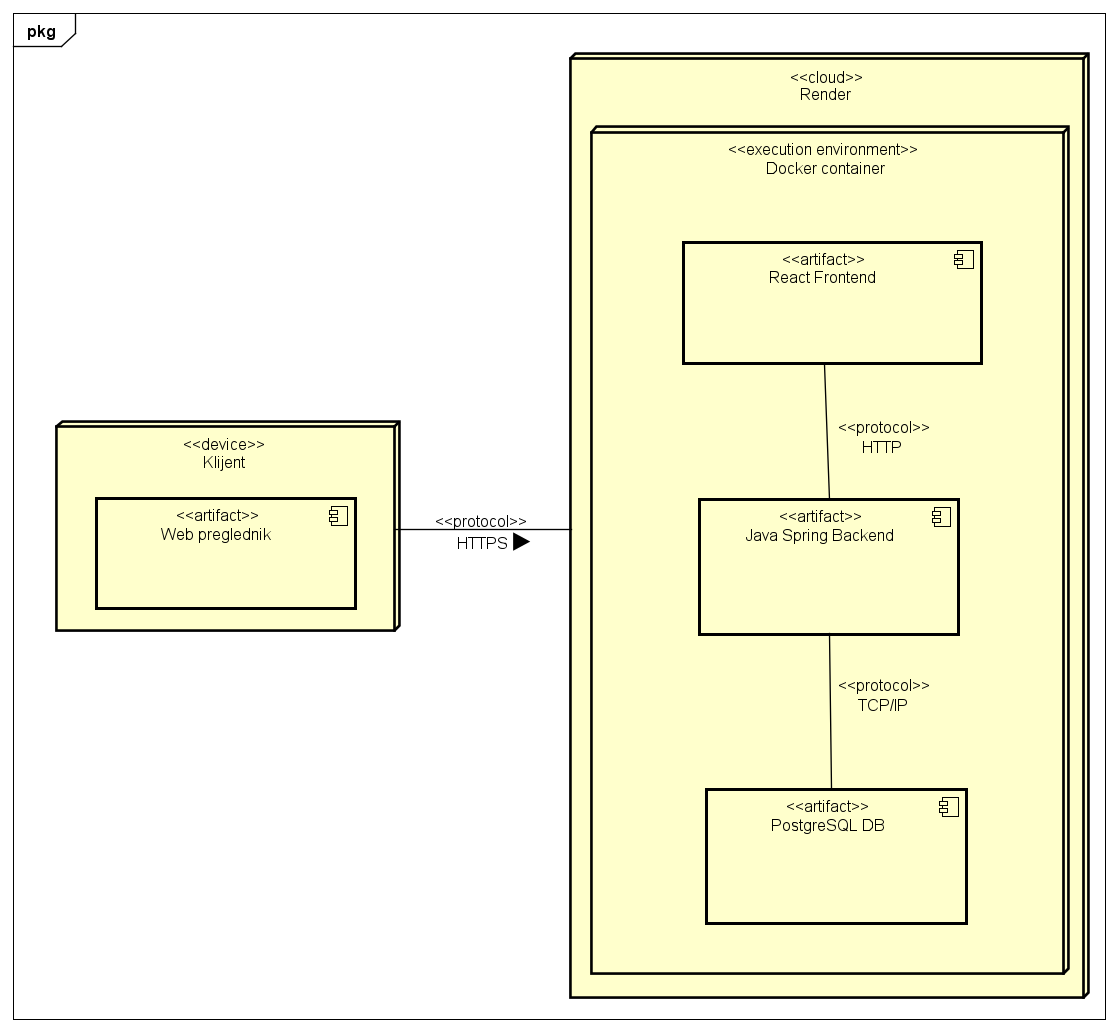
\includegraphics[width=\textwidth]{slike/DeploymentDiagram.PNG}
			 	\caption{Dijagram razmještaja}
			 	\label{fig:deploymentDiagram}
			 \end{figure}
			 
			 \newpage
			 
			 Slika 5.1 prikazuje dijagram razmještaja. Dijagram razmještaja prikazuje raspodjelu programskih komponenti kao što su izvršne datoteke i virtualna izvršna okruženja. Dijagram se sastoji od dvaju glavnih čvorova nazvanih Klijent i Render. Čvor Klijent predstavlja uređaj kojim klijent, odnosno korisnik pokušava pristupiti sustavu. Čvor se sastoji od jednog artefakta, Web preglednika. Web preglednik je izvršna datoteka kojom korisnik šalje sve zahtjeve u sustav i prima odgovore iz sustava. Drugi čvor na dijagramu je Render. Render je poslužiteljsko računalo/a koja su smještena u oblaku. Cijela aplikacija je smještena unutar kontejnera Docker u oblaku Render. Kontejner Docker je virtualno izvršno okruženje. Pripadni čvor Docker container je ugniježđen unutar čvora Render. Frontend dio aplikacije implementiran je kao React aplikacija, backend dio implementiran je koristeći Java Spring radni okvir, a baza podataka koja služi da pohranu svih potrebnih podataka implementirana je kao PostgreSQL. Komunikacija između korisnika, odnosno web preglednika i aplikacije odvija se preko HTTPS protokola, protokola na aplikacijskom sloju. Svaki od artefakata koji zajedno čine aplikaciju, međusobno komuniciraju. Komunikacija između frontend i backend dijela aplikacije izvodi se preko HTTP protokola, dok se komunikacija između Java Spring backenda i baze podataka izvodi s pomoću protokola nižih slojeva, točnije TCP/IP protokolima.
			
			\eject 
		
		\section{Upute za puštanje u pogon}
		
			\textbf{\textit{dio 2. revizije}}\\
		
			 \textit{U ovom poglavlju potrebno je dati upute za puštanje u pogon (engl. deployment) ostvarene aplikacije. Na primjer, za web aplikacije, opisati postupak kojim se od izvornog kôda dolazi do potpuno postavljene baze podataka i poslužitelja koji odgovara na upite korisnika. Za mobilnu aplikaciju, postupak kojim se aplikacija izgradi, te postavi na neku od trgovina. Za stolnu (engl. desktop) aplikaciju, postupak kojim se aplikacija instalira na računalo. Ukoliko mobilne i stolne aplikacije komuniciraju s poslužiteljem i/ili bazom podataka, opisati i postupak njihovog postavljanja. Pri izradi uputa preporučuje se \textbf{naglasiti korake instalacije uporabom natuknica} te koristiti što je više moguće \textbf{slike ekrana} (engl. screenshots) kako bi upute bile jasne i jednostavne za slijediti.}
			
			
			 \textit{Dovršenu aplikaciju potrebno je pokrenuti na javno dostupnom poslužitelju. Studentima se preporuča korištenje neke od sljedećih besplatnih usluga: \href{https://aws.amazon.com/}{Amazon AWS}, \href{https://azure.microsoft.com/en-us/}{Microsoft Azure} ili \href{https://www.heroku.com/}{Heroku}. Mobilne aplikacije trebaju biti objavljene na F-Droid, Google Play ili Amazon App trgovini.}
			
			
			\eject 
	\chapter{Zaključak i budući rad}
		
		\textbf{\textit{dio 2. revizije}}\\
		
		 \textit{U ovom poglavlju potrebno je napisati osvrt na vrijeme izrade projektnog zadatka, koji su tehnički izazovi prepoznati, jesu li riješeni ili kako bi mogli biti riješeni, koja su znanja stečena pri izradi projekta, koja bi znanja bila posebno potrebna za brže i kvalitetnije ostvarenje projekta i koje bi bile perspektive za nastavak rada u projektnoj grupi.}
		
		 \textit{Potrebno je točno popisati funkcionalnosti koje nisu implementirane u ostvarenoj aplikaciji.}
		
		\eject 
	\chapter*{Popis literature}
		\addcontentsline{toc}{chapter}{Popis literature}
	 	
 		%\textbf{\textit{Kontinuirano osvježavanje}}
	
		%\textit{Popisati sve reference i literaturu koja je pomogla pri ostvarivanju projekta.}
		
		
		\begin{enumerate}
			
			
			\item  Programsko inženjerstvo, FER ZEMRIS, \url{http://www.fer.hr/predmet/proinz}
			
			\item  I. Sommerville, "Software engineering", 8th ed, Addison Wesley, 2007.
			
			\item  T.C.Lethbridge, R.Langaniere, "Object-Oriented Software Engineering", 2nd ed. McGraw-Hill, 2005.
			
			\item  I. Marsic, Software engineering book``, Department of Electrical and Computer Engineering, Rutgers University, \url{http://www.ece.rutgers.edu/~marsic/books/SE}
			
			\item  The Unified Modeling Language, \url{https://www.uml-diagrams.org/}
			
			\item  Astah Community, \url{http://astah.net/editions/uml-new}
		\end{enumerate}
		
		 
	
	
	\begingroup
	\renewcommand*\listfigurename{Indeks slika i dijagrama}
	%\renewcommand*\listtablename{Indeks tablica}
	%\let\clearpage\relax
	\listoffigures
	%\vspace{10mm}
	%\listoftables
	\endgroup
	\addcontentsline{toc}{chapter}{Indeks slika i dijagrama}


	
	\eject 
		
	\chapter*{Dodatak: Prikaz aktivnosti grupe}
		\addcontentsline{toc}{chapter}{Dodatak: Prikaz aktivnosti grupe}
		
		\section*{Dnevnik sastajanja}
		
		%\textbf{\textit{Kontinuirano osvježavanje}}\\
		
		 %\textit{U ovom dijelu potrebno je redovito osvježavati dnevnik sastajanja prema predlošku.}
		
		\begin{packed_enum}
			
			\item  sastanak
			
			\item[] \begin{packed_item}
				\item Datum: 18.listopada 2023.
				\item Prisustvovali: J. Balatinec, I. Cvrk, V. Đurić, S. Kiš, A. Kućar, M. Štambuk, I. Žagar
				\item Teme sastanka:
				\begin{packed_item}
					\item  Inicijalni sastanak
					\item  Diskusija o početku rada
					\item  Upoznavanje sa zadatkom
				\end{packed_item}
			\end{packed_item}
			
			\item  sastanak
			
			\item[] \begin{packed_item}
				\item Datum: 25.listopada 2023.
				\item Prisustvovali: J. Balatinec, I. Cvrk, V. Đurić, S. Kiš, A. Kućar, M. Štambuk, I. Žagar
				\item Teme sastanka:
				\begin{packed_item}
					\item  Diskusija o radu s alatima za pisanje dokumentacije
					\item  Diskusija o stavljanju i preuzimanju na/s GitHub-a
					\item  Podjela rada za do sljedećeg sastanka
				\end{packed_item}
			\end{packed_item}
			
			\item  sastanak
			
			\item[] \begin{packed_item}
				\item Datum: 15.studenog 2023.
				\item Prisustvovali: J. Balatinec, V. Đurić, A. Kućar, I. Žagar
				\item Teme sastanka:
				\begin{packed_item}
					\item  Diskusija s demonstratoricom oko dosadašnjeg napretka na projektu
					\item  Diskusija o daljnjim koracima razvoja i zadacima na projektu
				\end{packed_item}
			\end{packed_item}
			
			\item  sastanak
			
			\item[] \begin{packed_item}
				\item Datum: 16.studenog 2023.
				\item Prisustvovali: J. Balatinec, I. Cvrk, V. Đurić, S. Kiš, A. Kućar
				\item Teme sastanka:
				\begin{packed_item}
					\item  Diskusija o svemu što je napravljeno na projektu
					\item  Dovršavanje implementacije i ispravak dokumentacije
					\item  Diskusija o daljnjem radu na projektu
				\end{packed_item}
			\end{packed_item}
			
			\item  sastanak
			
			\item[] \begin{packed_item}
				\item Datum: 13.prosinca 2023.
				\item Prisustvovali: V. Đurić
				\item Teme sastanka:
				\begin{packed_item}
					\item  Diskusija s demonstratoricom o prvom kolokviranju projekta
					\item  Diskusija s demonstratoricom o dijagramima obrazaca uporabe
				\end{packed_item}
			\end{packed_item}
			
			%
			
		\end{packed_enum}
		
		\eject
		\section*{Tablica aktivnosti}
		
			\textbf{\textit{Kontinuirano osvježavanje}}\\
			
%			 \textit{Napomena: Doprinose u aktivnostima treba navesti u satima po članovima grupe po aktivnosti.}

			\begin{longtblr}[
					label=none,
				]{
					vlines,hlines,
					width = \textwidth,
					colspec={X[7, l]X[1, c]X[1, c]X[1, c]X[1, c]X[1, c]X[1, c]X[1, c]}, 
					vline{1} = {1}{text=\clap{}},
					hline{1} = {1}{text=\clap{}},
					rowhead = 1,
				} 
			
				\SetCell[c=1]{c}{} & \SetCell[c=1]{c}{\rotatebox{90}{\textbf{Vinko Đurić}}} & \SetCell[c=1]{c}{\rotatebox{90}{\textbf{Josip Balatinec}}} &	\SetCell[c=1]{c}{\rotatebox{90}{\textbf{Ivan Cvrk }}} & \SetCell[c=1]{c}{\rotatebox{90}{\textbf{Stella Kiš }}} &	\SetCell[c=1]{c}{\rotatebox{90}{\textbf{Anđelko Kućar }}} & \SetCell[c=1]{c}{\rotatebox{90}{\textbf{Marina Štambuk }}} &	\SetCell[c=1]{c}{\rotatebox{90}{\textbf{Ivan Žagar }}} \\  
				Upravljanje projektom 		& 10 &  &  &  &  &  & \\ 
				Opis projektnog zadatka 	& 1 &  &  &  & 1 &  & 6 \\ 
				
				Funkcionalni zahtjevi       & 1 &  &  & 1 &  &  &  \\ 
				Opis pojedinih obrazaca 	& 7 &  &  & 3 &  & 2 &  \\ 
				Dijagram obrazaca 			& 9 &  &  & 1 &  &  &  \\ 
				Sekvencijski dijagrami 		&  & 6 &  &  &  &  &  \\ 
				Opis ostalih zahtjeva 		& 1 &  &  &  &  &  &  \\ 

				Arhitektura i dizajn sustava	 & 2 &  &  &  &  &  &  \\ 
				Baza podataka				& 6 &  &  &  &  &  &   \\ 
				Dijagram razreda 			& 6 &  &  &  &  &  &   \\ 
				Dijagram stanja				&  &  &  &  &  &  &  \\ 
				Dijagram aktivnosti 		&  &  &  &  &  &  &  \\ 
				Dijagram komponenti			&  &  &  &  &  &  &  \\ 
				Korištene tehnologije i alati 		& 1 &  &  &  &  &  &  \\ 
				Ispitivanje programskog rješenja 	&  &  &  &  &  &  &  \\ 
				Dijagram razmještaja			&  &  &  &  &  &  &  \\ 
				Upute za puštanje u pogon 		&  &  & 1 &  &  &  &  \\  
				Dnevnik sastajanja 			& 1 &  &  &  &  &  &  \\ 
				Zaključak i budući rad 		&  &  &  &  &  &  &  \\  
				Popis literature 			&  &  &  &  &  &  &  \\  
				&  &  &  &  &  &  &  \\ \hline 
				\textit{Frontend} 				&  &  & 10 &  &  &  & 21 \\  
				\textit{Backend} 		 			&  &  & 20 &  & 42 &  & \\ 
				\textit{Dizajn}				&  &  &  & 4 &  &  &  \\ 
			\end{longtblr}
					
					
		\eject
		\section*{Dijagrami pregleda promjena}
		
		\textbf{\textit{dio 2. revizije}}\\
		
		\textit{Prenijeti dijagram pregleda promjena nad datotekama projekta. Potrebno je na kraju projekta generirane grafove s gitlaba prenijeti u ovo poglavlje dokumentacije. Dijagrami za vlastiti projekt se mogu preuzeti s gitlab.com stranice, u izborniku Repository, pritiskom na stavku Contributors.}
		
	


\end{document} %naredbe i tekst nakon ove naredbe ne ulaze u izgrađen dokument 


